\documentclass[a4paper,12pt,oneside]{report}
\usepackage{a4wide}
\usepackage{ucs}
\usepackage[utf8x]{inputenc}
\usepackage{xcolor}
\usepackage[english,czech]{babel}
\usepackage[pdftex, final]{graphicx}
\usepackage{alltt}
\usepackage{paralist}
\usepackage{mdwlist}
\usepackage{subfig}
\usepackage[final]{pdfpages}
\usepackage[final,pdftex, colorlinks=false]{hyperref}
\usepackage{fancyhdr}
\usepackage[ruled,vlined]{algorithm2e}
%mensi mezera z figure
%\setlength{\belowcaptionskip}{-10pt}
\newcommand{\squeezeup}{\vspace{-2.5mm}}

\usepackage{enumitem}
\usepackage{url}

\usepackage{verbatim}
%\usepackage{pdfpages}
\usepackage{perpage} %the perpage package
%\MakePerPage{footnote} %the perpage package command

\usepackage{amsmath}
%\usepackage{hyperref}
\usepackage{acronym}
\usepackage[font=singlespacing]{caption}
\usepackage[font={small}]{caption}
\usepackage{multirow}
\usepackage{fancyvrb}
\usepackage{subfig}
\usepackage{titlesec}
\usepackage{listings}

\usepackage{footmisc}

\makeatletter
\def\verbatim@font{\linespread{1}\normalfont\ttfamily}
\makeatother

\usepackage{indentfirst}
\usepackage{wrapfig}

\usepackage{booktabs}

%%%%%%%%%% tabulka %%%%%%%%%%%

\usepackage{booktabs}
\usepackage{multirow}
\usepackage[normalem]{ulem}
\useunder{\uline}{\ul}{}
\usepackage{etoolbox}
\preto\tabular{\shorthandoff{-}}

%\usepackage{etoolbox}
%\patchcmd{\thebibliography}{\chapter*}{}{}{}

%cislovani kapitol
\renewcommand*\thesection{\arabic{section}}
\renewcommand{\chaptername}{}

%\titleformat{\chapter}{\normalfont\huge}{}{20pt}{\huge\textbf}

\renewcommand{\partname}{}
\renewcommand{\chaptername}{}


\setcounter{secnumdepth}{3}

%Abstract
\usepackage{lipsum}
\newenvironment{abstractpage}
  {\cleardoublepage\vspace*{\fill}\thispagestyle{empty}}
  {\vfill\cleardoublepage}
\newenvironment{abstractx}[1]
  {\bigskip\selectlanguage{#1}%
   \begin{center}\bfseries\abstractname\end{center}}
  {\par\bigskip}








%%%%%%%%%%%% rozmery %%%%%%%%%%%%%%%%%%
\usepackage[%
%top=40mm,
%bottom=35mm,
%left=40mm,
%right=30mm
top=40mm,
bottom=35mm,
left=35mm,
right=25mm
]{geometry}


\renewcommand\baselinestretch{1.3}
\parskip=0.8ex plus 0.4ex minus 0.1 ex

%%%%%%%%%%%%%% Listings %%%%%%%%%%%%%%%%%

\definecolor{lightGrey}{RGB}{250,250,250}
\definecolor{darkGrey}{RGB}{230,230,230}
\lstdefinelanguage{psmap}
{morekeywords={scale, mapinfo, maploc, where, end, font, fontsize, color,
border, raster, width, paper,
vpoints, vareas, vlines, symbol, size, rgbcolumn, sizecolumn, cwidth,
rotatecolumn, },
morekeywords=[2]{y, n, none},
morecomment=[l]{\#},
}

\lstdefinestyle{XML}{
  language=XML,
  basicstyle={\ttfamily\scriptsize},
  morekeywords={encoding,
    xs:schema,xs:element,xs:complexType,xs:sequence,xs:attribute}
}

\lstdefinestyle{script}{
    language=bash,
    basicstyle={\ttfamily\footnotesize},
    keywordstyle={\bfseries},
    commentstyle={\itshape},
    %frame=lines,
    backgroundcolor=\color{lightGrey}
}


\lstdefinestyle{mybash}{
   language=bash,
   basicstyle={\ttfamily\scriptsize},
   keywordstyle=[1]{\bfseries},
   keywordstyle=[2]{\color{black}},
   commentstyle={\itshape},
   frame=lines,
   showstringspaces=false,
   %backgroundcolor=\color{darkGrey},
}

\lstdefinestyle{python}{
   language=python,
   basicstyle={\ttfamily\scriptsize},
   keywordstyle=[1]{\bfseries},
   keywordstyle=[2]{\color{black}},
   commentstyle={\itshape},
   frame=lines,
   showstringspaces=false,
   %backgroundcolor=\color{lightGrey},
}





%%%%%%%%%%%%%%%%%%%%%%%%%%%%%%%%%
\newcommand{\klicslova}[2]{\noindent\textbf{#1: }#2}
\newcommand{\modul}[1]{\emph{#1}}
%\newcommand{\instr}[1]{\lstinline[style=psmapInline]|#1|}
\author{Matěj Krejčí}
% \pagecolor{darkGrey}
\newcommand{\necislovana}[1]{%
\phantomsection
\addcontentsline{toc}{section}{#1}
\section*{#1}
\markboth{\uppercase{#1}}{}
}


%%%%%%%%%%%%%%%%%%%%%%%%%%%%%%
\begin{document}
\pagestyle{empty}




\renewcommand{\bibname}{References}
\renewcommand{\contentsname}{Content}
\renewcommand{\figurename}{Fig.}
\renewcommand{\tablename}{Tab.}




%nastaveni velikosti footnote
\renewcommand\footnotelayout{\footnotesize}
\pagenumbering{gobble}


\begin{center}
%napisy
\newcommand{\napisCVUT}{Czech Technical University in Prague}
\newcommand{\napisFS}{Faculty of Civil Engineering}
\newcommand{\napisProgram}{Geodesy and Cartography}
\newcommand{\napisObor}{Geomatics}
\newcommand{\napisKatedra}{Department of Geomatics}
\newcommand{\napisVedouci}{Ing. Martin Landa, Ph.D.}
\newcommand{\napisAutor}{Bc. Matěj Krejčí}
\newcommand{\napisDatum}{Prague 2016}
\newcommand{\napisNazevI}{Processing of vector data using distributed}
\newcommand{\napisNazevII}{database systems in GIS}
\newcommand{\napisNazevAjI}{Využití distribuovaných databázových}
\newcommand{\napisNazevAjII}{ systémů pro správu vektorových dat v GIS}
\newcommand{\napisBakalarka}{Master thesis}
\newcommand{\napisPraha}{Prague 2016}
%
% prikazy
%\newcommand{\velka}[1]{\uppercase{#1}}
\newcommand{\velka}[1]{\textsc{#1}}
%
% 
\newif\ifpatitul
\patitultrue

\ifpatitul
{\Large\velka{\napisCVUT}}\\
\velka{\Large\napisFS}\\
\vfill
{\LARGE\velka{\napisBakalarka}}
\vfill
{\large\napisPraha\hfill\napisAutor}
\newpage
\fi%patitul


{\Large\velka{\napisCVUT}}\\
{\Large\velka{\napisFS}}\\
{\Large\velka{\napisProgram}}\\
{\Large\velka{\napisObor}}\\
\vfill

\includegraphics[width=3cm]{logo_cvut_cb} %~
\vfill

{\Large\velka{\napisBakalarka}}\\
{\Large\velka{\napisNazevI\\
\napisNazevII}}\\
{\large\velka{\napisNazevAjI\\
\napisNazevAjII}}
\vfill
{\large%
Supervisor: \napisVedouci\\
\napisKatedra\\
\bigskip
\napisDatum\hfill\napisAutor}
\end{center}


\begin{abstractpage}
\begin{abstractx}{czech}

  CIL..


  \klicslova{Klíčová slova}{GIS, GRASS}
\end{abstractx}

\begin{abstractx}{english}

	Aim of...

  \klicslova{Keywords}{GIS, GRASS}
\end{abstractx}
\end{abstractpage}




\newpage
\newcommand{\odsaditodzhora}{\hskip1pt\vfill}

\odsaditodzhora
\noindent {\bf Declaration of authorship}

\vskip 1.5 \baselineskip

I declare that the work presented here is, to the best of my knowledge and
belief, original and the result of my own investigations, except as acknowledged.
Formulations and ideas taken from other sources are cited as such.

\begin{flushleft}
\begin{tabular}{cp{0.3\textwidth}c}
In Prague .................
& 
&
..................................
\\
&&
(author sign)
\end{tabular}

\end{flushleft}
\newpage

\odsaditodzhora
\noindent {\bf Acknowledgment}

\vskip 1.5 \baselineskip

I would like to thank my parents for their support during my studies.
Great gratitude, I would like to express Martin Landa, my supervisor, for giving sense to my university studies.
\newpage

\newpage

\setcounter{tocdepth}{3}

\tableofcontents
%\addtocontents{toc}{~\vspace{-3\baselineskip}}


\newpage
\necislovana{Introduction}

\pagestyle{fancy}
\fancyhf{}
\renewcommand{\sectionmark}[1]{\markboth{#1}{}} % set the \leftmark
\fancyhead[L]{CTU in Prague}
\fancyhead[R]{\leftmark} % 1. sectionname
\fancyfoot[C]{\thepage}


\pagenumbering{arabic}
\setcounter{page}{1}
\subsection*{Context}
%Over the years the capabilities of hard drives have increased massively and access speed too. According to study by International %Data Corp, since 2007 we produce more data than we can store. This amount of data is widely named big data.
\subsection*{Motivation and contribution}

\subsection*{Aim of the thesis}

 



\newpage
\chapter*{Background of related work}\stepcounter{chapter}\addcontentsline{toc}{chapter}{Background of related work}
\paragraph*{Starter}

\section{Hadoop framework}
\label{sec:hadoop}
		\subsection*{Hadoop}
		\emph{"The Apache Hadoop software library is a framework that allows for the distributed
		  processing of large data sets across clusters of computers using simple programming 
		  models. It is designed to scale up from single servers to 
		 thousands of machines, each offering local computation and storage. Rather than rely 
		 on hardware to deliver high-availability, the library itself is
		  designed to detect and handle failures at the application layer, so delivering a 
		  highly-available service on top of a cluster of computers,
		  each of which may be prone to failures."}(Apache Hadoop,\cite{hadoop_web})
 \begin{figure}[!htbp]
    \centering
    
\includegraphics[width=0.3\textwidth]{./img/664px-Hadoop_logo.png}
    \caption[Hadoop architecture2]{\centering Hadoop Logo.}
 \end{figure}
		
		\paragraph*{History}goes back to 2002 when the 
open-source project Apache Hadoop software for reliable, scalable,
distributed computing was launched. The project was originally
developed within Yahoo! company. That was the first company
which used framework Hadoop in production environments.

 
At the beginning of October 2003, Hadoop project was launched to improve performance
of the Apache Nutch\cite{nutch_web} web search engine and in the short time (in January 2006) was moved to the new Hadoop sub project.
At the same time  distributed file system called Google
file system\cite{google_fs}, with the specific, permitting, efficient and reliable access
the huge amount of data, has been created. This abstract file system, widely called "user level"
file system runs as a service that is accessible via APIs and libraries. 
In 2008, Hadoop was mad own top-level project at Apache.\cite{hadoop_web_news} By this time, Hadoop was being used by many
other companies besides Yahoo!, such as Last.fm, Facebook, and the New York Times. 

 \begin{figure}[!htbp]
    \centering
    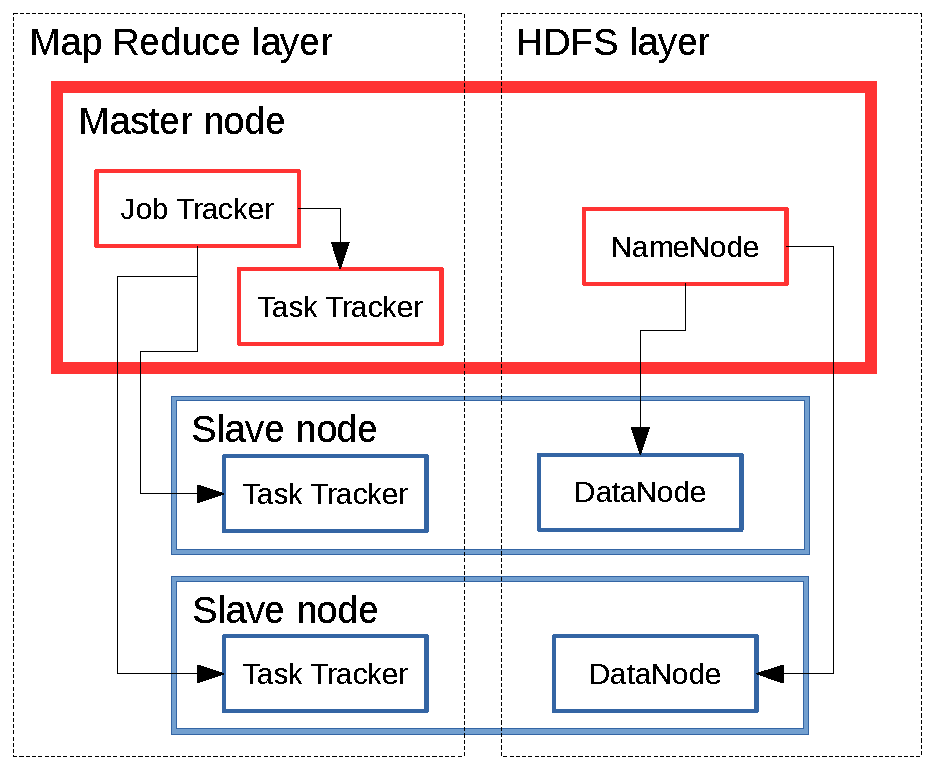
\includegraphics[width=0.6\textwidth]{./img/schema2.pdf}
    \caption[Hadoop architecture2]{\centering Hadoop HDFS and MapReduce layers}
 \end{figure} 
 
 
 
\paragraph*{The base Apache Hadoop}framework written in Java is composed of the following modules(Hadoop Apache \cite{hadoop_web}):
\begin{itemize}
\item \textbf{Hadoop Common} - The common utilities that support the other Hadoop modules;
\item \textbf{Hadoop Distributed File System (HDFS)} – A distributed file system that provides
 high-throughput access to application data;
\item \textbf{Hadoop YARN} - A framework for job scheduling and cluster resource management;
\item \textbf{Hadoop MapReduce} - an implementation of the MapReduce programming model 
for large scale data processing.
\end{itemize}
All the modules in Hadoop are designed with a expectation that hardware failures  are common and thus 
must be automatically managed by the architecture of  software.

The Hadoop framework is written in Java with some native code in C and command line utilities written 
as shell-scripts. But for development \textit{Map} and \textit{Reduce} parts of the user's program  
with "Hadoop Streaming" any programming language. 
Beside main modules, there are many Hadoop extensions for cluster management, 
data access and helpers for storing data in HDFS. As suitable example of this theses is Apache Hive, 
which expose higher level user interfaces and provide like SQL query syntax. 

There are two primary components at the core of Apache Hadoop 1.x: the Hadoop Distributed File System 
(HDFS) and the MapReduce parallel processing framework. For Hadoop 2.x have been developed new MapReduce 
framework named YARN, which handling better the week point of MapReduce v.1.


		\subsection{HDFS: Hadoop Distributed File System}\label{subsec:hdfs}
As the main source for describing HDFS have been used the official documentation (\textit{hadoop.apache.org} 
\cite{hadoop_web}) and book (\textit{Hadoop: The Definitive Guide}\cite{hadoop_definitive})

\paragraph*{Hadoop} comes with a filesystem and since it manages the storage of files on several 
machines, it is called Hadoop Distributed FileSystem (HDFS). Is designed for handling very large files with streaming
data access.\cite{hadoop_hdfs_web} In HDFS, large files are broken down into smaller blocks (128MB, by default) which are 
stored as independent units. The architecture of HDFS is a highly fault-tolerant and provides wide permeability
for access.   
  A short overview of main characteristics of HDFS design is described in (Hadoop: The Definitive 
  Guide\cite{hadoop_definitive}) as five features: (1)\textbf{Very large files} - With relevant hardware data of amounts petabytes 
can be accessed on Hadoop clusters effectively. (2) \textbf{Streaming data access} - Efficient data processing is based on
 read once and copied many times pattern. (3)\textbf{Commodity hardware} is suitable for running Hadoop. At the end,
 this fact helped with the decision to invest value of money to the development of Hadoop instead 
 of operating on expensive and highly reliable hardware. (4) \textbf{Low-latency data access} - HDFS is not suitable for performing
 low-latency access to data. Primary, HDFS is optimized for delivering
a high throughput of data. (5)\textbf{Lots of small files} allows to read and operate over more files
 at the same time. Limitation of number of stored directories,  files and block in filesystem is limited by \emph{Namenode} memory.

HDFS is based on traditional hierarchical file model. As in other filesystems, HDFS allows basic file operations: 
read, write, rename, move etc. However it doesn’t support hard and soft links. Below is the example of copying file between HDFS folders. 
\vskip-2ex
\begin{footnotesize}
\begin{lstlisting}[style=mybash]
$ hadoop fs -cp /user/hadoop/file1 /user/hadoop/file2 
\end{lstlisting}\end{footnotesize} 

\begin{figure}[!htbp]
    \centering
    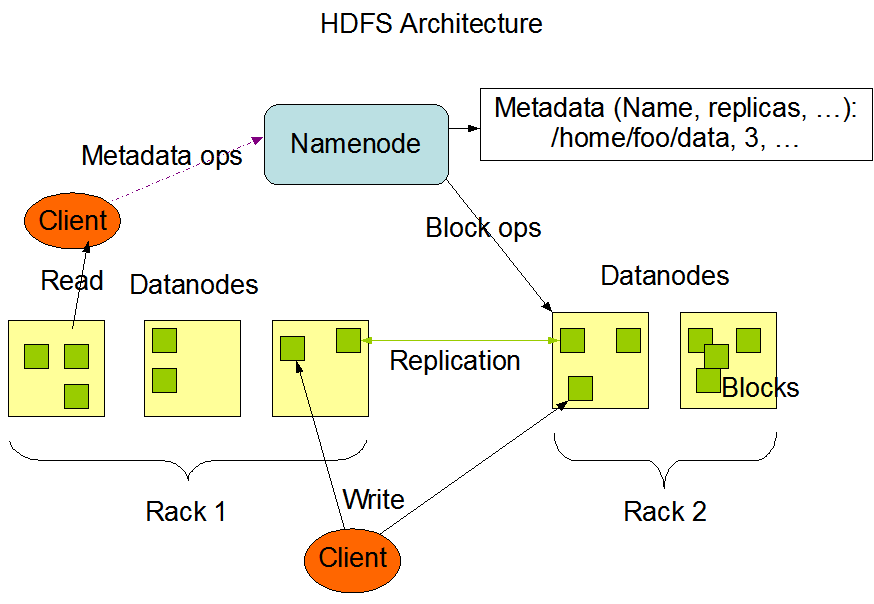
\includegraphics[width=1\textwidth]{./img/hdfsarchitecture.png}
    \caption[HDFS architecture1]{\centering HDFS architecture \footnotemark}
\end{figure} 
 \footnotetext{Figure source: \url{https://hadoop.apache.org/docs/r1.2.1/hdfs_design.html}}

		\subsubsection{Organization of data}
Similarly to  a common filesystem, HDFS is based on the disk blocks as well. The traditional
file system is based on blocks which define the minimal size of the amount of data to read and write.
HDFS blocks have the similar concept based on blocks, but the minimal unit is
larger. The size of the block is 128 MB by default. Blocks are broken and distributed
over disks on the cluster like blocks over a single disk in the filesystem. The ideal 
size of stored files is the same as the size of the block. With increasing the block 
size time cost for computing increases as well. On the other hand, a large number
of blocks is expensive for the preparation of files. The important task is to find the optimized 
ratio between the data preparation and the computational time by set suitable blocks size.
The idea of block abstraction helps to bring several benefits. First advantages of
abstraction design which allows storing bigger file than physical disk unit, 
even the fact that for Hadoop it is unusual.

The second benefit of fixed size is simplifying of storage management. Obviously, it is easy task
to hold calculating of size discernibility and eliminating metadata concerns (not necessary 
to store metadata of tree in data blocks, even in the same system.)
Furthermore, the blocks are suitable for replication and for providing fault tolerance. Protection
against corrupted blocks, disks or machines is based on replication of block over a cluster. 
Moreover, this approach ensures the integrity of HDFS checksums when reading as well as reading data.

\textbf{Replication selection process} is suited to minimize bandwidth consumption over a cluster. 
To minimize read latency, HDFS is primary try to read the closest replica to the reader. Priority is the 
same rack as node reader. \cite{hadoop_hdfs_web}

\textbf{Rack Awareness} on Hadoop serves for getting the maximum potential of production, 
it means that it knows the network topology. The purpose of rack-aware replication is ensured by policy 
component. It controls data reliability, availability, and network bandwidth. For a multi-rack cluster, is suitable to need to map 
nodes to a rack\cite{hadoop_rack_web}. This can be ensured manually or using program for mapping hierarchy of IP 
addresses. The priority of transfers is a size of bandwidth availability.  Within transfers 
where there is more bandwidth available as compared to off-rack transfers for MapReduce jobs on a node. 
By theory, the better network bandwidth is between machines in the same rack, due to hardware specifics.
		
		\subsection{Hadoop server components}
Hadoop architecture can be categorised into Client Machines, Master Servers and Slave Servers. These are basically daemons or programs that run on different physical servers. Hadoop consists five main components: 
\begin{itemize}[noitemsep]
\item NameNode
\item DataNode
\item Secondary NameNode
\item JobTracker
\item TaskTracker
\end{itemize}

\paragraph{Client}
computers have installed Hadoop with  all the configuration but they are not hosted on Master or Slave 
server. The Clients task is to  load data into the cluster, submit jobs and get the result or looking for jobs when finished.
		
		\subsubsection{NameNode, DataNode and SecondaryNameNode}
Hadoop comes with cluster architecture based on master(\textit{Namenode}) and\\ slave(\textit{DataNode}) design pattern. 
The \textit{NameNode} handles metadata of abstract file system(namespace), which include
information about the structure of files and directories in the tree.  It does not hold any cluster data itself. 
The  \textit{NameNode} only knows blocks which make up a file and where those blocks are located in the cluster.
Information about filesystem is stored on local disk in two files: the namespace image and edit log file. 
The \textit{NameNode} know all locations of  \textit{DataNodes} blocks where data 
are stored. It also provides the primary user interface to access HDFS. 
By design \textit{NameNode}  is a single point of failure and should be never overloaded and must 
be the most reliable node of the cluster.  Without \textit{NameNode}, HDFS is totally unserviceable. 

In recent Hadoop releases, there is also a backup node - \textit{SecondaryNameNode}, always up to date 
with latest(per 1 hour by default) \textit{NameNode} status. It receives all the operations done by \textit{NameNode} and 
stores them in local memory. This permits to have the latest, up to date namespace status, when \textit{NameNode} fails. 
        
As has been mentioned, the blocks of a file are independently stored in nodes, which are called
\textit{DataNodes}. Every \textit{DataNode} in the cluster makes registration process to the \textit{NameNode} during start. 
Besides that, each \textit{DataNode} informs \textit{NameNode} about blocks availability by sending a block report. 
Block reports are sent periodically or when a change event happens. Moreover, every \textit{DataNode} sends 
\emph{relevant} messages to the \textit{NameNode} to confirm that
it remains operational and that the data is safe and available. If a \textit{DataNode} stops operating, the error 
mechanisms designed to defend the failure and data loss maintain the availability of the block.
\emph{Relevant} messages also hold information, which allows the \textit{NameNode} to run the cluster efficiently e.g. 
load balancing. One important concept of design  is that \textit{NameNode} never directly calls data.
		

\subsubsection{JobTracker and TaskTrackers}
Above the file systems is  the MapReduce layer, in other words, MapReduce engine, which consists of 
JobTracker,  which ensures client applications to submit MapReduce jobs. The JobTracker handle work 
out to available TaskTracker nodes in the cluster, 
aiming to keep the jobs close to a data block.  Thus, JobTracker and TaskTracker are two types of 
nodes for managing the execution process of  task.
Client submits MapReduce job  to the JobTracker to process a particular file. JobTracke chose the 
DataNodes which store block with the desired file by asking the NameNode which store metadata of filesystem. 
JobTracker appends tasks to TaskTracker according to the  information obtained from NameNode and monitors the status of each task.


\subsection{HDFS access} %TODO check grammar
Several ways how to use HDFS interactively are available. In analogy to file system,  is  the main task to move data from local data to HDFS, access it and remove. As in standard file system, in HDFS is provided permission model as well. In paragraphs below are described access methods to HDFS and permissions models.

\paragraph{Permission model}
The permission model of HDFS has several levels. The level of files and directory similar to POSIX model. Each file and directory is associated with an owner and a group. Each item in HDFS, such a file and directory has separate permission. Thus, individual permissions for the user, that is a user, for other users that are member of group and the rest of users. Permission are: r for reading, w for writing and x not for execution, but for permission to access a child of the directory.\cite{permission}

There are two different models for checking the user's identity.
\begin{itemize}
\item \textbf{simple}  In this model is the identity of user derived from host operating system.
\item \textbf{Kerberos} In Kreberos model, is managed the identification process by Kerberos credentials system which is based on 'tickets' to allow nodes communicating over a non-secure network to prove their identity to one another in a secure manner.\cite{kerberos}
\end{itemize}

The identity mechanisms are  extrinsic to HDFS itself. Thus, within HDFS is not handler for creating user identities, establishing groups, or processing user credentials.

\paragraph{Access tools}
The basic mechanism to contraction with HDFS is \textit{hadoop fs}  command line tool. 
\begin{footnotesize}
\begin{lstlisting}[style=mybash]
bin/hadoop fs <args>
\end{lstlisting}
\end{footnotesize}
All fs shell commands take path URIs as arguments. Most of the commands in FS shell are derived from Unix commands. 

The other mechanism for accessing HDFS is through application programming interfaces such a APIs: Native Java API, which has a base class \textit{org.apache.hadoop.fs\\.FileSystem}; C API that works through the \textit{libHDFS} library, and there's a header file, \textit{hdfs.h} which has information on the API calls.

In addition there is REST API which widely used with connection to World Wide Web. REST is an architectural style consisting set of rules and constraints applied to components within distributed system. The WebHDFS REST API components fully cover the standard fs tool. The API consists four main groups of HTTP requests, such as: HTTP GET for fetching information, HTTP PUT for manipulation request, HTTP POST for append or concat file and HTTP DELETE for deleting files and directories.\cite{rest_api}
The Unix tool \textit{curl}  allows to access API from the Unix terminal. The example below demonstrate submit  HTTP POST request using the URL in the Location header with the file data to be appended.
\begin{footnotesize}
\begin{lstlisting}[style=mybash]
$ curl -i -X POST -T <LOCAL_FILE> "http://<DATANODE>:<PORT>/webhdfs/v1/<P..."
\end{lstlisting}
\end{footnotesize}
The client receives a response with zero content length:
\begin{footnotesize}
\begin{lstlisting}[style=mybash]
HTTP/1.1 200 OK
Content-Length: 0
\end{lstlisting}
\end{footnotesize}

	\subsection{Parallel computing - MapReduce}		
The \emph{MapReduce} is a programming model for processing and generating large data
sets. The \emph{MapReduce} abstraction is inspired by the Map and Reduce functions, which is commonly
found in functional programming languages, such as LISP \cite{lisp}. Users can easily express their
computation as a series of Map and Reduce functions. The Map function processes a series of
\textit{$<$ key, value $>$} pairs to generate a set of intermediate \textit{$<$ key, value $>$} pairs.

\begin{center}
Map(keyA, valueA) → list (keyB, valueB)
\end{center}
Reduce function aggregates all intermediate values that associate to the same intermediate key
to produce the final output, also in the form of $<$ key, value $>$ pairs
\begin{center}
Reduce(keyB, list(valueB)) → list (key C, valueC)
\end{center}
Thus the \emph{MapReduce} framework transforms a list of (key, value) pairs into a list of values. 


\paragraph{As MapReduce demonstration} in this work the use of data from cellular microwaves links(MWL)  is suitable . 
Assuming that data are already serialized and stored in text files and each file representing 24 hours 
of captured data, the size amount of weakly data is relatively small(~100Mb) which is adequate.
We are interesting in computational of then  mean differences between transmitted and received signal for 
each link in the period between 2014-07-07 and 2015-07-07.

Below is the sample of data stored as CSV.
\begin{footnotesize}
\begin{lstlisting}[style=mybash]
linkid;data;rx;tx
324;"2014-07-07 11:14:56.552";-48.9;10
256;"2014-07-07 11:14:59.703";-99.9;7
...
324;"2015-07-07 17:10:56.578";-50.1;7;
256;"2015-07-07 17:10:56.484";-85.3;10;
\end{lstlisting}\end{footnotesize}
 
The text lines above are presented to map functions as key-values pairs.
The map function extracts data from date 2014-07-07 and creates pairs {link:(rx-tx)}
\begin{footnotesize}
\begin{lstlisting}[style=mybash]
{324:-58.9}
{256:-106.9}
...
{324:-57.1}
{256:-95.3}
\end{lstlisting}\end{footnotesize}


The output is processed by MapReduce framework before is being sent to reduce function.
Mentioned process sorts pairs by key as shown bellow.
\begin{footnotesize}
\begin{lstlisting}[style=mybash]
{324:[-58.9,-57.1]}
{256:[-106.9,-95.3]}
\end{lstlisting}\end{footnotesize}


Finally reduce program iterates over the list of values for each link and compute mean.
 The final results are stored in Hadoop file system.
 


\section{Spatial processing in parallel}
	\subsubsection{Introduction to Spatial MapReduce Query}
Figure \ref{fig:mapred_spatial} shows a simple example of distributed spatial query processing. The main idea 
grows up from the basis of MapReduce. On the figure, the dataset is partitioned into four tiles. After 
query job is started each tile is analyzed separately using Map(M1-M4) function. For demonstration, 
query analyzes intersection of two datasets(red, blue) on each tile and relation between 
objects from the different dataset is detected. The result is done by Reduce(R) function, where results from each
map phase are processed.

\begin{figure}[h!]
    \centering
    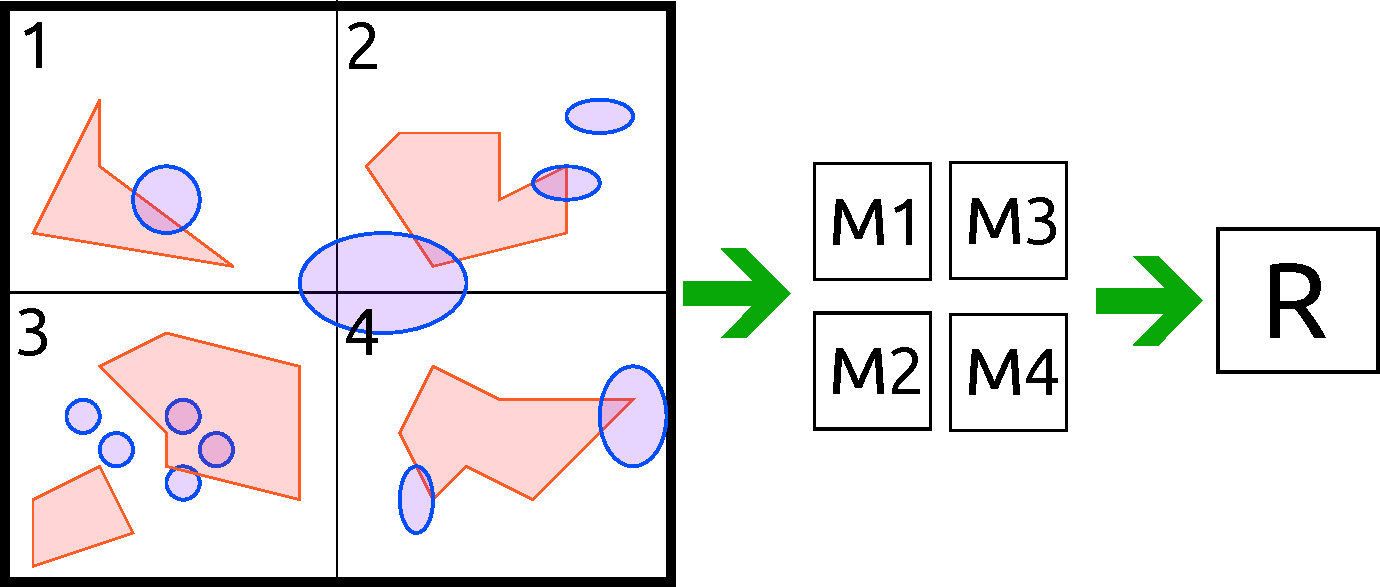
\includegraphics[width=0.5\textwidth]{./img/mapred_spatial.pdf}
    \caption[Spatial Map Reduce]{\centering Detection of spatial relations using Map(\textit{M1-M4}) and Reduce(\textit{R}) functions}
        \label{fig:mapred_spatial}
 \end{figure}
\paragraph{}

The motivation for spatial processing in parallel is queering data in reasonable time. 
Firstly, it is essential to introduce characteristics of queries for solving different 
tasks. In HadoopGIS (F. Aji, F. Wang, et al.\cite{hadoopGIS}) there is defined five major 
query cases of spatial data: (1) \textit{Feature Aggregation queries}  which doesn’t 
fall into spatial queries, however, they are evenly important for spatial frameworks 
as others. As a common example of Feature Aggregation query, a function for finding mean 
values of attributes. 
\textit{Fundamental Spatial Queries} covers groups of tasks like: including point based 
queries, containment queries, and spatial joins. (3) Next groups 
\textit{ Complex Spatial Queries} includes more challenging task. A query which solves 
advanced Spatial Join: spatial mismatching or overlay; or neighbor query. (4) Integrated 
spatial and feature queries, which combine query from more categories, such feature 
aggregation queries in a selected spatial regions. Finally (5) \textit{Global
Spatial Pattern Queries}, for example, queries on finding high-density regions, or 
queries to find directional patterns of spatial objects.

Anyway, classification of a query to five groups is based on characteristics of a task. 
But, as in RDBMS as well in distributed databases, the most challenging is to solve  cost-intensive query. 
Join Queries and Nearest Neighbour queries can be classified as 
cost-intensive to compare to the rest and because of that, it becomes as interesting and
most challenging task for a scientist, developers. Logically that fact affects the direction of the most of academic works and developments.

Speeding up a process of solving \textit{Spatial Join} which is classified as classic GIS 
problem is a motivation for the parallel processing of spatial data. Spatial Join 
is an operation used to combine two or more datasets with respect to a spatial 
relationship. Detection of relations between spatial objects using serial(used in RDBMS) 
computing approach started to be limited by its design. On the scene comes solutions
based on parallel and distributed models. In the past, many distributed 
solutions as OpenMP\cite{omp} have been presented, for instance, Intel TBB and Bulk Synchronous Parallel\cite{multi_cpu}.
Because of their complexity, they have been used insignificantly to compare with Hadoop framework.
Already introduced MapReduce parallel model opens doors for developing efficient
spatial query engine with less developing investments. In the last years,  
few projects came up on the scene  focused on Spatial MapReduce.
\textit{SpatialHadoop}\cite{spatialhadoop}, \textit{HadoopGIS}\cite{hadoopGIS} and \textit{ESRI Spatial Framework for Hadoop}\cite{esri_framework}
are three open source systems that are designed to process large scale spatial data on Hadoop.
All three systems come with significantly different design of implementation but they all are based
on Map Reduce framework from Hadoop environment and basically all project have the same goal.
To realize such systems, it is essential to identify time-consuming spatial query components,
break them down into small tasks, and process these tasks in parallel. 
Design of first two systems, \textit{SpatialHadoop} and \textit{HadoopGIS}
extensions are well described in publications. Background of Esri library is not described in an available
publication, on the other hand, the user documentation seems to be complex and described in detail. 
Esri laboratory published article\cite{esri_indexing} about QuadTree indexing, which is used for building 
indexes in their \textit{ESRI Spatial Framework for Hadoop}.
In the section below there are described fundamentals of spatial processing in parallel and the in discussion 
the comparison of solutions of developed and published frameworks is provided. The main source for description 
of frameworks is mentioned literature (\textit{SpatialHadoop}\cite{spatialhadoop}, \textit{HadoopGIS}\cite{hadoopGIS} 
and \textit{ESRI Spatial Framework for Hadoop}\cite{esri_framework})

		
\subsection{Spatial Join}
\label{sub:spatial_join}
Assume two sets of multi-dimensional object in \emph{Euclidean space}. Relation of spatial 
join between sets \emph{R} and \emph{S} can be defined\cite{spatial_join2}:

\begin{center}
$R\bowtie_{pred}S=\left \{ \left ( r,s|r  \right )\in R,s \in S, pred(r,s) is \ \ true) \right \}  $
\end{center}
where $\bowtie_{pred}$ is a spatial predicate for the relationship of two
spatial objects. 
\linebreak 
\textit{Spatial join} finds all pairs of object which satisfying a spatial relation between given objects. 
For further explanation of the spatial join concept assume that  objects \emph{s} from set \emph{S} and 
analogically  \emph{r} from \emph{R} are rectangles. Intersection operation between each rectangle \emph{s} 
and \emph{r} will report set \emph{R} of intersected \emph{r} rectangles.

Solution of described \textit{spatial join} is trivial. General spatial join problem has been extended by 
complex spatial join, known as \textit{spatial overlay join}\cite{spatial_join}: (a)The set of objects
can be another character than a rectangle, such as point, segments or polygon. (b) The dimension of a set 
can be more than three. (c) The relationship between pairs of objects may be any relationship between 
objects which includes spatial elements, such as intersections, nearness, enclosure, or a directional relation. 

To speed up spatial join query different ways based on filtering are commonly used.
Typical trivial solutions are covered by usage of Minimal Bounding Box (MBB) as a first 
filter for defining the subset of candidate object satisfying a spatial predicate. For defining of MBBs for 
sets of points Convex Hull algorithm can be used. 
To speed up computation the construction of Convex Hull based on heuristic \cite{covex_hull} is more efficient. 
In Spatial Join technique \cite{spatial_join} 
many different methods of filtering spatial objects and their suitability for specific 
requirements are used. For large dataset stored in GIS, the filtering is essential. The object such a polygon 
or point cloud can reach millions or more features. Boolean vectors operation on detecting relation without filter stage 
can be extremely expensive in a meaning of I/O performance. Usually, in the first stage is filtering data; spatial objects 
are read from hard drive which is sufficient for computation of MBRs, then created MBRs are 
stored in memory and the spatial join test is performed faster.


		\subsubsection{Spatial Data Partitioning}
		\label{Spatial_Data_Partitioning}
Data partitioning is a powerful mechanism for improving an efficiency of data management systems, 
and it is a standard feature in modern database systems. Partitioning data into smaller units allows 
for query processing in parallel and further improved performance. In addition,
with proper partition scheme, I/O operations may be substantially
reduced by scanning only a few sections that contain relevant information to answer a question.
By architecture of Hadoop design, the important step and the first one is defining a suitable format for 
storing data which influences  speed of their access and at least query process. In general, the 
partitioning produces sub-datasets based in smaller regions-tiles is the common approach.
There are two main reasons for the partitioning of spatial data. 
The first one is to avoid tiles with high density. This is mainly due to the potential high 
skew\cite{spatial_skew} of data which could imbalance workers in a cluster environment. Another aspect is to  
properly handle boundary of intersecting objects. As MapReduce provides custom
scheduling  for balancing tasks the problem of load imbalance can be partially 
mitigated to a task of scheduling planning. In work (Effective Spatial Data Partitioning for Scalable Query 
Processing \cite{partitioning}) has been introduced and compared six methods of spatial data partitioning for parallel processing. 

\begin{figure}[h!]
    \centering
    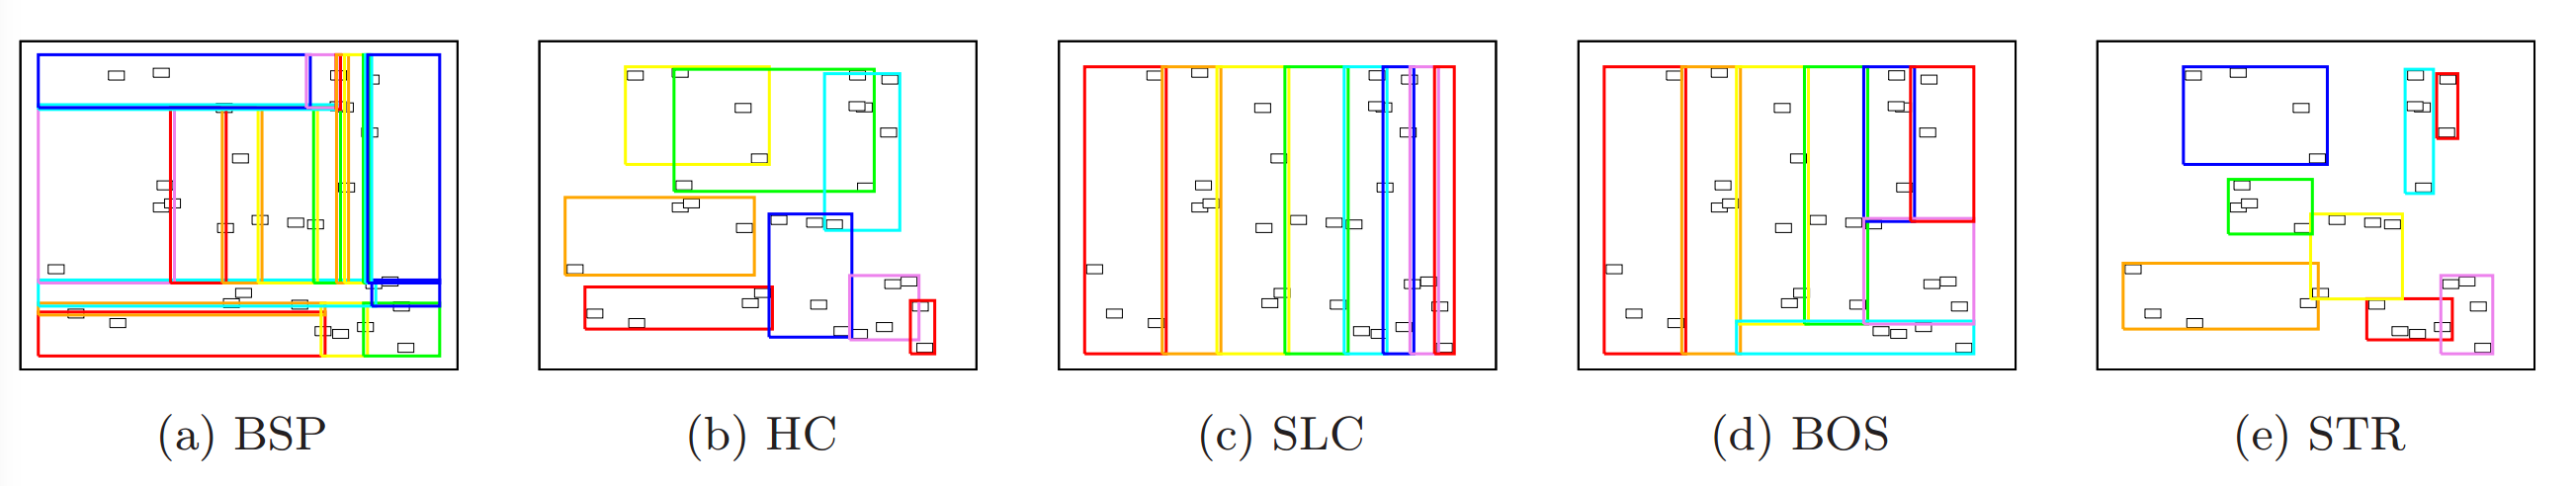
\includegraphics[width=1\textwidth]{./img/part_overview.png}
    \caption[mapreduce flow]{\centering  Spatial partitions generated by different algorithms BSP: Binary split 
    partitioning, FG: Fixed grid
partitioning, SLC: Strip partitioning, BOS: Boundary optimized strip partitioning, STR: sort-tile-recursive
partitioning, HC: Hilbert curve partitioning. Source of fig: \cite{partitioning}}
 \end{figure} 

\paragraph{Spatial Data skew} is common in a spatial application. Example \cite{hadoopGIS} assumes dataset of 
$1000\cdot1000$ tiles. The maximum count of the object is 10 000 objects, but the average count is $1020$. This 
fact growing from the real situation where a high density of objects are e.g. in cities and less dense in farmlands. 
In parallel spatial processing where a distribution of processes is based on tiles, the data skew can significantly 
increase the response time.

\paragraph{Boundary object}
Spatial partitioning generates boundary objects that cross multiple partitions. Thus, it influences the independent relation 
of each partition. In a usual case, a spatial object has complex boundary and extent. Even more, 
from real experience is evident that in spatial datasets spatial object can cross multiple partitions. The problem is solved with 
different methods; replicating spatial object to multiple partitions and filtering duplicates during query process 
or another approach, creation sector with putting weight on minimizing boundary objects. 

\paragraph*{} \textbf{HadoopGIS} in partitioning stage is focused on breaking high-density tiles into smaller ones, with using 
recursive partitioning. Firstly, they provide two-dimensional data partitioning and generates a set of tiles.
These preprocessed tiles are a source for query tasks. The preprocessing is done with the using of distributed computing.
 Week point of tile-based approach is non-adaptable algorithm on non-uniformly distributed data. Because that, 
 in practice with spatial partitioning the critical problem of \textit{data skew} is known. HadoopGIS ensures 
 this problem by cutting high-density tiles into small ones thus recursive partitioning approach. For controlling 
 number of objects per tile  maximal and a minimal number of objects per tile is defined. Splitting recursion 
 finds optimal direction(x or y) for creating half-sized tiles which fulfil the thresholds by a number of objects 
 in each half. In HDFS storage, the final tiles are not stored in small files taking into account default HDFS blocks size (128MB). 

\paragraph*{} \textbf{SpatialHadoop} implemented the solution  based on the same tiles based idea as HadoopGIS, but few features 
are significantly different.
The main difference is storing partitions (tiles) in HDFS blocks instead in a big batch file. Algorithm for creating tiles differently 
is  based on that. Three main characteristics arise from that fact. SpatialHadoop is counting 
with a size of HDFS block and the size of tiles should fit  that size. It avoids data skew of spatial datasets. 
Secondly, a design of partitioning method ensures spatial locality; a spatially close object is assigned to the same 
partition. The last feature tempts to balancing the size of a partition. In an ideal case, all partition are the 
same size. The number of partitions \emph{n} is computed as $n=\left[ \frac{S(1+ \alpha)}{B}\right]$,
 where \emph{S} is the size of input file, \emph{B} is the HDFS block size and $\alpha$ is an overhead ratio(0.2 by default). 
 Next step is the definition of boundaries by of partitions. Boundaries are represented by rectangles. Thus, a skew of data is not considered. 
 The output of this step is set of rectangles representing  boundaries of partition. Together it represents cover 
 of whole space domain. The result is input for initialization of physical partitioning procedure. The method solving 
 the problem of an object with spatial extents (e.g. polygon) which overlaps more than one partitions. Determination 
 of solution is based on selected index methods; when some of them assign object to all overlapping partitions and 
 the others find the best matching partition. Replicated records are managed later by  query processor. Finally, 
 for each record from partition the map function write the pair $<$partition,record$>$ which are grouped by 
 partitions and sent to reduce function for the next task- indexing phase.


		\subsubsection{Spatial Indexing}
		\label{Spatial_Indexing}
One essential requirement for spatial queries is a fast response. 
In general, the filtering and partitioning  of spatial objects are widely related to indexing. 
Spatial indexing helps to avoid to sequential browsing in other words to avoid full table scanning.
Generally, in RDBMS for creation index over specified column or multiple columns is available multiple 
indexing methods like btree, hash, gist, and gin. On spatial indexing problem in RDBMS have 
been done many scientific works and different algorithms have been shown. Suitability of 
different indexing methods is linked to the characteristics and distribution of data. 
Adaptation of serial indexing method to parallel processing quite challenges. 
RDBMS has the ability to use information from multiple indexes to determine how best
to search for the records that satisfy all query criteria. A
NoSQL key-value store, in contrast, has only a single index
that is built atop the constraint that all records are ordered
lexicographically . Traditional 
Spatial Indexes from the field of RDBMS e.g. Grid file or R-tree are not suitable for parallel 
processing. By design of traditional indexing method, they are not designed for effective 
usage on Hadoop, where developers implement indexing in a procedural way and the execution 
runs on multiple threads. Since Hadoop is based on MapReduce layer to implement 
sequential construction instead of incremental one  is necessary.  
MapReduce is a scan based data processing framework which does not utilize any form of a disk-based 
index and the performance is limited as the input has to be scanned. The design of spatial indexing methods 
is according to filtering approach and choose a partitioning pattern. 



\paragraph*{} \textbf{SpatialHadoop} indexing model is composed from three phases. The first phase, partitioning is already
described\ref{Spatial_Data_Partitioning}.

The purpose of the second phase is to build \textit{local index}  for each physical partition of data. 
In contrast to global index, the local index is built for each partition sparely. In addition, each local 
index is stored in on one HDFS block. It ensures that Hadoop uses load balancer for relocating blocks 
across machine. Additionally, it allows  a spatial operation to access local indexes where each local 
index is processed in one map task. 

Last phase, building the \textit{global index} provide index structure of all partitions. As next step, 
 all local indexes to one file which represent the final index of spatial data are concatenated. This process 
provides using MapReduce parallel framework.  After this part is done the NameNode creates a global index
and store it in memory. The index is based on dictionary; key and value.

\begin{footnotesize}
\begin{lstlisting}[style=mybash]
-179.3248215,-54.934357,6.9290401,71.2885321,part-00000_data_00001
-171.773529,-54.81145,6.9261512,65.1480999,part-00000_data_00001_1
6.9225032,-46.44586,179.3801209,78.0657531,part-00000_data_00002_2
\end{lstlisting}\end{footnotesize}


 Key is represented by HDFS block and  rectangular boundaries as value. This index keeps all the 
 time in the main memory. That ensure faster access. In critic situation when fail of master or 
 restart of a cluster is possible to rebuild index from rectangular boundaries of the file blocks. 
 For accessing the master index is not necessary to parse it yourself. Implantation offers API 
 which retrieves the global index as an object.
SpatialHadoop offers tree methods for building indexes. 

The simple one, \textbf{Grid Index} is a flat and partitions of
data according to a grid such that records overlapping each grid cell are stored in one file block 
as a single partition. Grid index is suitable for uniformly distributed data. Otherwise, the data 
screw is critical by the principle of MapReduce. 

Besides grid index, SpatialHadoop framework offer building index based on method \textbf{R-tree} and 
\textbf{ R+-tree}. Fig \ref{fig:partitioning} (b) shows results of R-tree algorithm. 

  \begin{figure}[h!]
	\centering
    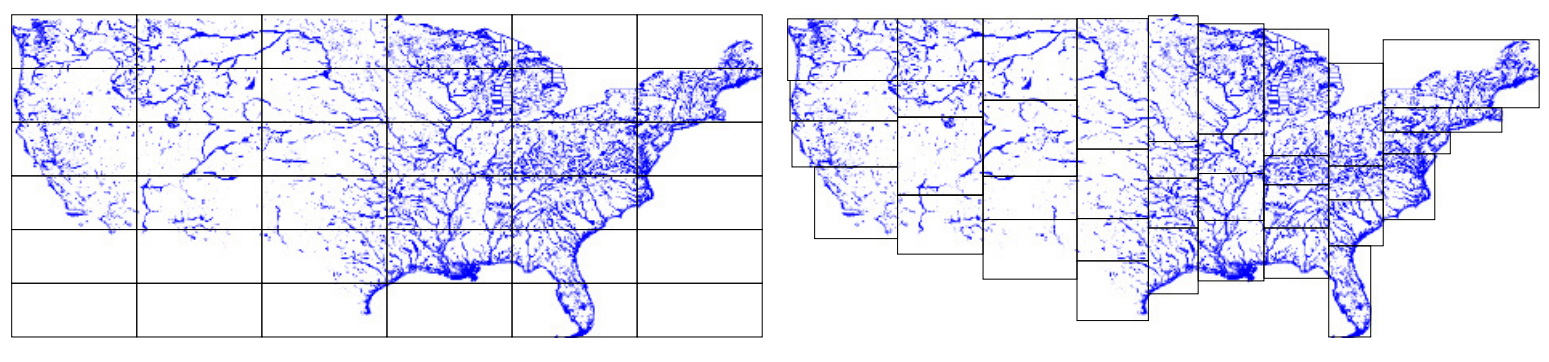
\includegraphics[width=1\textwidth]{./img/spatial_hadoop_parti.png}
    \caption[Spatial Map Reduce]{\centering (a) Grid Partitioning (b) R-tree Partitioning.\footnotemark}
    \label{fig:partitioning}
  \end{figure}  
\footnotetext{Source: SpatialHadoop: A MapReduce Framework for Spatial Data; Eldawy A., Mokbel,F.M \cite{spatialhadoop} }
    
\paragraph*{} \textbf{HadoopGIS} indexing is based on hierarchical space partitioning and MBB based 
region filtering. Similarly, to Grid Index of SpatialHadoop design is built from  combination of local 
indexes and global index. Recursively each tile can be further partitioned into even smaller regions. 
But, HadoopGIS does not pre-generate indexes into files. Finally, HadoopGIS supports uniform grid 
index, which is efficiently applicable only in the rare case of uniform data distribution. 

		\subsection{Spatial Operation}


TODO in progress!
\paragraph{Interface}Three mentioned spatial processing frameworks (section \textit{Spatial Join}\ref{sub:spatial_join}) 
for Hadoop show different design for storing and accessing data. Similarly, the interface for 
configuration, data management and query data varies.

Operation on \textit{HadoopGIS} and \textit{Spatial frameworkGIS from Esri are based} are based on likeSQL layer. 
Concretely on the top of spatial MapReduce library Hadoop extension is implemented, likeSQL data warehouse- Hive.  
\textit{SpatialHadoop} supports spatial extension Pigeon a high level SQL-like language which  provides OGC-compliant 
spatial data types and operations making it easier to adopt by users. It makes the program simpler and more expressive 
as it uses spatial data types (e.g. POINT and RECTANGLE) and spatial functions (e.g. Overlaps). 
The spatial functionality is implemented as user defined functions (UDFs) which are seamless to integrate with existing 
non-spatial operations in Pig.
		
		
		TODO
		  ogc spatial operators

		  popsat customizaci SpatialHadoop
	      https://github.com/aseldawy/spatialhadoop2/wiki/Implementing-custom-spatial-operations-in-SpatialHadoop
 		  https://github.com/Esri/spatial-framework-for-hadoop/wiki/UDF-Documentation
		  https://cwiki.apache.org/confluence/display/Hive/Spatial+queries






\begin{table}[!htbp]
\begin{footnotesize}
\centering
\begin{tabular}{@{}|c||c|c|c|@{}}
\toprule
framework    & HadoopGIS   & SpatialHadoop    & \begin{tabular}[c]{@{}c@{}}Spatial framework \\ for Hadoop(Esri)\end{tabular}         
                                                                     \\ \midrule \midrule
\begin{tabular}[c]{@{}c@{}}integration \\ with extension\end{tabular} & HiveSP                                                                           & \begin{tabular}[c]{@{}c@{}}Pigeon(spatial \\ extension for\\  Apache Pig)\end{tabular} & Hive                                                                                                                                                                   \\ \midrule
\begin{tabular}[c]{@{}c@{}}build-in\\ data types\end{tabular}         & \begin{tabular}[c]{@{}c@{}}Point, Polygon, \\ Box and \\ LineString\end{tabular} & \begin{tabular}[c]{@{}c@{}}Point, Rectangle\\ and Polygon\end{tabular}                 & \begin{tabular}[c]{@{}c@{}}inherit from\\ Esri Java Geometry \\ Library: Point, MultiPoint, \\ Polyline, Polygon, Envelope.\\ Also includes OGC Wrappers.\end{tabular} \\ \midrule
input data                                                            & CSV                                                                              & \begin{tabular}[c]{@{}c@{}}CSV,\\ custom \\ data types\end{tabular}                    & Json                                                                                                                                                                   \\ \midrule
\begin{tabular}[c]{@{}c@{}}User-defined\\ data types\end{tabular}     & -                                                                                & \begin{tabular}[c]{@{}c@{}}- for Pigeon\\ + SpatialHadoop\end{tabular}                 & -                                                                                                                                                                      \\ \midrule
visualisation                                                         & -                                                                                & +*HadoopViz                                                                            & \begin{tabular}[c]{@{}c@{}}*Geoprocessing \\ Tools for Hadoop\\ (ArcMap)\end{tabular}                                                                                  \\ \midrule
index                                                                 & \begin{tabular}[c]{@{}c@{}}uniform grid\\  index\end{tabular}                    & R-tree,R+-tree,Grid index & QuadTree                                                                                                                                                               \\ \midrule
\begin{tabular}[c]{@{}c@{}}accessible\\ index\end{tabular}            & -                                                                                & +                                                                                      & -                                                                                                                                                                      \\ \bottomrule

\end{tabular}
\caption{Overview of spatial frameworks for Hadoop}
\label{tab:comparison_spatial_fr}
\end{footnotesize}
\end{table}
	
		\subsection{Summary}\ref{summary_libs}
		
 SpatialHadoop, HadoopGIS and ESRI Spatial Framework for Hadoop are
three open source systems that are designed to process large scale
spatial data on Hadoop. Although the features of  the implementation of each framework are different, 
the overall design is suited to Map and Reduce function principals. Spatial cross join is well suited to parallelizable and fit to MapReduce. 

All three spatial frameworks come with indexing, where SpatialHadoop is the most customizable. 
The design of  SpatialHadoop implementation is open to extending available indexes. Esri and 
SpatialHadoop offer more advanced indexing methods, such as 
QuadTree(Esri) and E-tree(SpatialHadoop). One of the main weakness of HadoopGIS is an indexing 
support. It disposables only by grid index method which can be 
effectively used only for uniformly distributed data.

To compare with others, SpatialHadoop comes with the different MapReduce approach for solving cross-spatial join.
In SpatialHadoop, both sides in a spatial join are partitioned and its implemented as only 
Map job.  SpatialHadoop makes pairs from spatially overlapping partitions, which are finally 
assigned to Map tasks for parallel and distributed execution.

In addition, SpatialHadoop implements filtering using MapReduce as a preprocessing step.
HadoopGIS as a first step join both datasets, reorder and assign its data to the same 
HDFS block.  Accessing data are provided by key-value pairs. Partitions are represented by keys and item as values. 

When decision which framework is suitable for a specific application must be made, the 
key factor can be access of data  or programming language choice. While SpatialHadoop 
uses binary format for representation data in memory and disk, HadoopGIS 
uses Hadoop streams. Thus, HadoopGIS representing all side results as text and access 

of data is only sequential. In contrast, SpatialHadoop binary approach allows 
accessing data randomly.
These facts make SpatialHadoop more efficient since parsing text are an expensive task. 
On the other hand, HadoopGIS allows writing MapReduce function in different languages than Java which can be crucial. 


Generally, all frameworks allow customization on the level of developing MapReduce functions. As Esri 
framework allows interaction with core libraries, is more focused  for GIS users than developers. 
Esri covers the wide portfolio of built-in spatial operators to compare SpatialHadoop framework, 
and at least significantly more than HadoopGIS. On the other hand, the leader for customization and 
development of additional functionality is SpatialHadoop.


\begin{table}[!htbp]
\begin{scriptsize}
\centering
\begin{tabular}{@{}|l||l|l|@{}}
\toprule
Group                       & Framework                                                        & Description                                                                                                                                                  \\ \midrule \midrule
\multirow{5}{*}{Compute}    & Compute engine                                                   & large-scale workloads on virtual machines                                                                                                                \\ \cmidrule(l){2-3} 
                            & Preemptible VMs                                                  & short-lived instances for batch and fault-tolerant jobs                                                                                                  \\ \cmidrule(l){2-3} 
                            & Custom Machine Types                                             & customized deployment of virtual machine                                                                                                                 \\ \cmidrule(l){2-3} 
                            & App Engine                                                       & engine for building scalable web app and mobile backends                                                                                                 \\ \cmidrule(l){2-3} 
                            & Container engine                                                 & powerful cluster manager for running Docker containers                                                                                                   \\ \midrule
\multirow{5}{*}{Storage}    & Cloud storage*                                                   & simple, cost effective data storage                                                                                                                       \\ \cmidrule(l){2-3} 
                            & \begin{tabular}[c]{@{}l@{}}Cloud storage\\ Nearline\end{tabular} & highly-durable storage for data archiving and online backup                                                                                              \\ \cmidrule(l){2-3} 
                            & Cloud SQL                                                        & storing data using relational MySQL database                                                                                                             \\ \cmidrule(l){2-3} 
                            & Datastore   \ref{subsub:datastore}                               & scalable, NoSQL database for non-relational data                                                                                                         \\ \cmidrule(l){2-3} 
                            & Bigtable                                                         & fast, scalable NoSQL database service                                                                                                                    \\ \midrule
Networking                  & Cloud networking                                                 & load balancing, VPN, DNS,                                                                                                                                \\ \midrule
\multirow{5}{*}{Big Data}   & BigQuery                                                         & real time analysis(100,000 rows)of data per second                                                                                                       \\ \cmidrule(l){2-3} 
                            & DataFlow                                                         & real-time data processing for batch and stream data processing                                                                                           \\ \cmidrule(l){2-3} 
                            & Dataproc\ref{subsub:dataproc}                                                        & management for Spark and Hadoop services. Quick deployment                                                                                               \\ \cmidrule(l){2-3} 
                            & DataLab                                                          & analysis and visualisation of large-scaled data                                                                                                          \\ \cmidrule(l){2-3} 
                            & Pub/Sub                                                          & \begin{tabular}[c]{@{}l@{}}real-time messaging service for sending up to\\ 1 milion messages per second\end{tabular}                                     \\ \midrule
\multirow{2}{*}{Services}   & Cloud Endpoinds                                                  & API for access to backend servers for mobile platforms                                                                                                   \\ \cmidrule(l){2-3} 
                            & Translate API                                                    & allows to develop apps for translating languages programatically                                                                                         \\ \midrule
\multirow{4}{*}{Management} & Cloud monitoring                                                 & monitoring performance and availability of cloud apps                                                                                                    \\ \cmidrule(l){2-3} 
                            & Cloud deployment manager                                         & manager for repeatable deployment using templates                                                                                                        \\ \cmidrule(l){2-3} 
                            & Container registry                                               & private Docker image storage                                                                                                                             \\ \cmidrule(l){2-3} 
                            & Cloud logging                                                    & \begin{tabular}[c]{@{}l@{}}Mannager for log data and engine for debug system issue.\\ Supports Google App Engine and Google Compute Engine.\end{tabular} \\ \bottomrule
\end{tabular}
\end{scriptsize}
\caption{Overview of Google Cloud platform}
\label{tab:google_all}
\end{table}


		
	\section{Google Cloud Platform}
\textbf{Cloud} in IT field generally means deploying an application and running it on a platform which is 
provided by someone else. Services allow to developers  work efficiently  with 
requisite resources which are necessary for an application to work.

\textbf{Google cloud platform}, supports building, testing and deploying an application on highly-scalable 
infrastructure.
The platform is based on building blocks. Advantages of design the platform design is a quick development of 
desired product by combining separate services together. Portfolio of services is sorted into six main categories 
which are described for better overview in 
table\ref{tab:google_all} \cite{gc_product_services}.

The user interface offers three different ways for managing services of Google Cloud. Web-based interface, command-line 
interface and programming API. The most user-friendly interface is web based. The web interface provides to 
user quick overview and a better understanding of 
options over each service. On the other hand, the range of configuration possibilities is limited compared with the rest 
interfaces. \textit{Google Cloud SDK} is a 
package of tools for managing resources and application on Google Cloud Platform. 
Package includes \textit{gcloud tool} for Google Compute Engine resources and \textit{gsutil} for working with Cloud Storage.



\paragraph{Command-line interface} called \textit{gcloud} enables to manage Google Compute Engines resources in faster way 
to compare with Compute Engine API. It uses concept of configurations for managing different accounts on Google Cloud. 
Interface of \textit{gcloud} is suited for handling services of Google cloud platform using command line. For example, 
deploying VM, handling containers, configuring network and the other.
%\vskip-2ex
%\begin{figure}[!htbp]
%\lstset{extendedchars=false,escapeinside=''}
%\begin{footnotesize}

\begin{lstlisting}[style=mybash]
%$ gcloud config configurations create my-config
%\end{lstlisting} 

%\vskip-3ex
Configuration allows to set default general variables: account, project, default region 
and zone, proxy etc. To set up configuration profile: default zone, region is appropriate. 
The variables can be set by \textit{gcloud} or with using 
local variables.
Below is an example of deploying VM instance with default configuration. The instance 
is accessible by \textit{gcloud} ssh tool(e.g. instance run in zone asia-east1). Access can be also provided 
by standard ssh protocol.

\begin{footnotesize}
\begin{lstlisting}[style=mybash]
$ gcloud compute instances create my-instance
...
$ gcloud compute ssh my-instance --zone asia-east1
...
\end{lstlisting}\end{footnotesize}
 

\textit{gcloud dataproc}\ref{subsub:dataproc} tools support deployment of clusters with limited configuration. For deploying 
clusters with distributed file system, like Hadoop and spark, is suitable to use \textit{bdutil}\ref{sub:bdutil} tools. 
This example demonstrate, that command line tools doesn’t fully cover full portfolio of Google Cloud Platform. 
   
\paragraph{Google Cloud Client Libraries} give programmatic access to Google Cloude Platform services. For development of applications 
linked to cloud services it ensure better language integration, security handling and easy general access. Libraries are currently 
available in five languages: Go, Java, Note.js, Python and Ruby. Below is shown 
example of Python API library. In this case the sample of code allows to initialize  
instance of Cloud Dataproc and get JSON object represented list of clusters.

\begin{footnotesize}
\begin{lstlisting}[style=python]
from oauth2client.client import GoogleCredentials
project = 'my-test-project'
region = 'global'
credentials = GoogleCredentials.get_application_default()
result = dataproc.projects().regions().clusters().list(
         projectId=project,
         region = region).execute()
\end{lstlisting}\end{footnotesize}
 


		\subsection{Geography and Regions}
Google cloud platform is available across three \textit{locations}: North America, Europe, and Asia. Each location includes 
\textit{regions} and \textit{zones}. The choice of place, where service is running is on developer. The statistics of data 
center resources; latency availability, durability are available and the with using API allows to manipulated with resources problematically. 
%\begin{figure}[h!]
%\centering
%	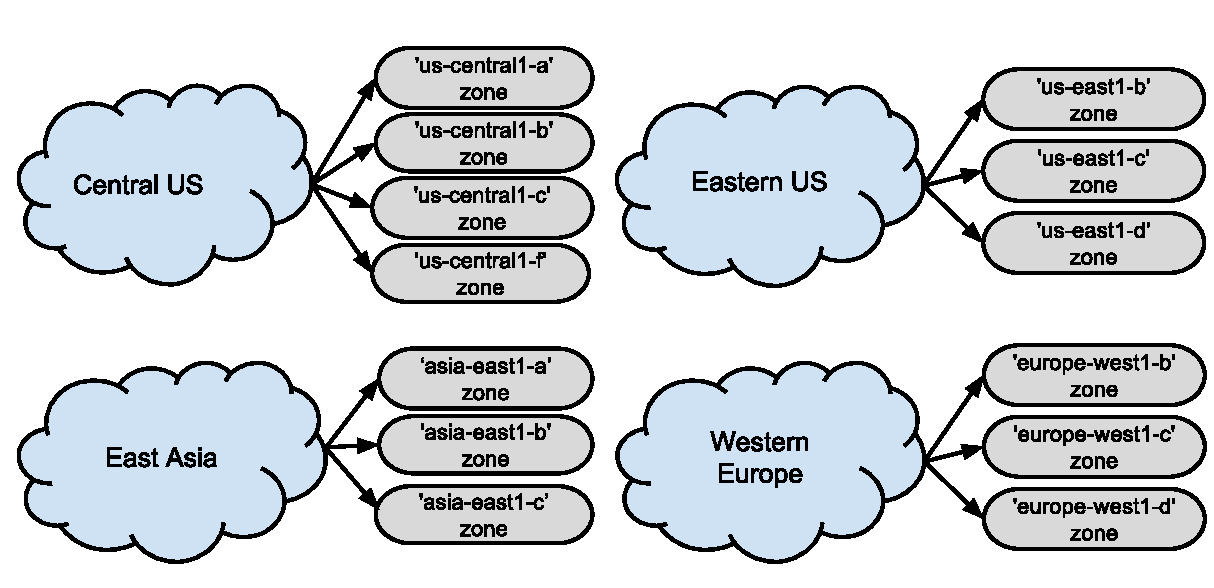
\includegraphics[width=0.7\textwidth]{./img/zones_diagram.pdf}
%    \caption[Spatial Map Reduce]{\centering Zones diagram describing zones available in each region\footnotemark}
%    \label{fig:partitioning}
%  \end{figure}  
%\footnotetext{Source:\url{https://cloud.google.com/compute/docs/zones}}

\paragraph*{Hierarchy}
Design of network is suited to ensures maintenance  of custom services efficiently. The hierarchical model provided separated
 levels of failure as well as room for distributing resources across multiple regions or zones. Main abstract unit is \textit{location} 
 which consists \textit{regions}. To ensure availability, locations are independent to each other important features of locations is the 
 network latency under 5ms on the 95th percentile. Lower level of hierarchy, thus subset is \textit{zone}. As well as location, 
 zones are independent to each other. Location consists of zones which should be classified as single point of failure. Thus, 
 to build up fault-tolerant application is necessary to deploy it over different zones. Furthermore, to choose region according 
 to geographic location of accessing points is suitable. In addition, to ensure fail of service on the level of \textit{region}, 
 Google suggests to have a backup plan for migration to another one. Fully qualified address of zone   for API access is \textless 
 region\textgreater-\textless zone\textgreater \ e.g. \textit{europe-west1-d}. 


\begin{footnotesize}
\begin{lstlisting}[style=mybash]
## view list of available zones.
$ gcloud compute zones list
NAME           REGION       STATUS NEXT_MAINTENANCE 
asia-east1-c   asia-east1   UP
..

## check available regions.
$ gcloud compute regions list
NAME         CPUS         DISKS_GB    ADDRESSES RESERVED_ADDRESSES STATUS 
asia-east1      0.00/8.00      0/2048      0/23      0/1           UP
..

## get information about desired zone e.g asia-east1.
$ gcloud compute regions describe asia-east1
creationTimestamp: '2014-05-30T18:35:16.514-07:00'
description: asia-east1
id: '1220'
kind: compute#region
name: asia-east1
quotas:
- limit: 8.0
  metric: CPUS
  usage: 0.0
..
\end{lstlisting}\end{footnotesize}
 
        



\subsection{Identity and Access Management}
Cloud Identity and Access Management(Cloud IAM) provide another way for handling privacy 
and permissions for \textit{Google Cloud} services. Currently, alpha  or beta versions are 
supported for nine services over Google Cloud portfolio, 
includes \textit{Google Cloud Storage}. IAM design is based on three main pillars, 
such as \textit{Roles}, \textit{Policy} and \textit{Resources}. The 
identity of a user is handled by four different authentication methods such a Google 
account, Service account, Google group and Google Apps domain.

\paragraph{Resources} Allowed grant access to users for Cloud Platform resources. Thus 
to available services of Google Cloud portfolio. To allow permissions for using given 
service is declared syntax \textless service\textgreater.\textless resource\textgreater.\textless verb\textgreater, for example \emph{pubsub.topics.publish}.

\paragraph{Roles} A role represent the collection of permissions. Two kinds of the role 
are available, such as Primitive roles and Curated roles. The first mentioned, concentric 
roles, thus, Owner role can also Edit and Edit role includes 
Read role. This basic role approach is applied e.g. in Cloud Storage as default. Second, 
curated roles are new and allow more advanced policy management. 
Currently(28.3.2016), \textit{Curated roles}(\ref{fig:iam}, (a)) are in alpha or beta 
development version and are not suggested to use for production 
use. However, these Curated roles provide additional granular access to specific services 
from Google Cloud portfolio and prevent unwanted access to 
other resources. In figure
% Please add the following required packages to your document preamble:
% \usepackage{booktabs}
\begin{table}[!htbp]
\begin{scriptsize}
\centering
\begin{tabular}{@{}|l|l|l|@{}}
\toprule
Role                        & Description                                                                                                                         & Permissions                                                                        \\ \midrule \midrule
roles/storage.objectCreator & \begin{tabular}[c]{@{}l@{}}Allows users to create objects. \\ Does not give permission to delete or overwrite objects.\end{tabular} & storage.objects.create                                                             \\ \midrule
roles/storage.objectViewer  & \begin{tabular}[c]{@{}l@{}}Grants access to view objects and\\ their metadata, excluding ACLs.\end{tabular}                         & \begin{tabular}[c]{@{}l@{}}storage.objects.get\\ storage.objects.list\end{tabular} \\ \midrule
roles/storage.objectAdmin   & Grants full control of objects.                                                                                                     & storage.objects.*                                                                  \\ \midrule
roles/storage.admin         & Grants full control of objects and buckets.                                                                                         & \begin{tabular}[c]{@{}l@{}}storage.buckets.*\\ storage.objects.*\end{tabular}      \\ \bottomrule
\end{tabular}
\caption{Cloud Storage Roles covered by IAM}
\label{iam}
\end{scriptsize}
\end{table}
	

\paragraph{Policy} of Cloud IAM can grant roles to users. It is designed as a collection 
of statements that specify who has what type of access. The policy is linked to resources 
and control it's accessed. In figure(\ref{fig:iam}, (b)) is 
shown policy principle based on the relation between the collection of statements IAM and 
Resources of Google Platform. Resources of Google Platform 
are organized hierarchically. Figure (\ref{fig:iam}, (c)) demonstrated example of the nodes 
in hierarchy. \textit{Organisation} represent the root of 
the hierarchy and each child has only one parent. Inheritance of hierarchy allows handling 
in easy way sets and subsets of abstract classes, such as Organization, Project and Resources. 


\begin{figure}[!htbp]
    \centering
    %\subfloat[Roles]{ 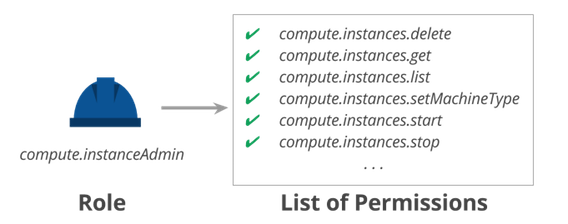
\includegraphics[width=0.4\textwidth]{./img/iamroles.png} }%
    %\qquad
    %\subfloat[Cloud IAM policy management]{ 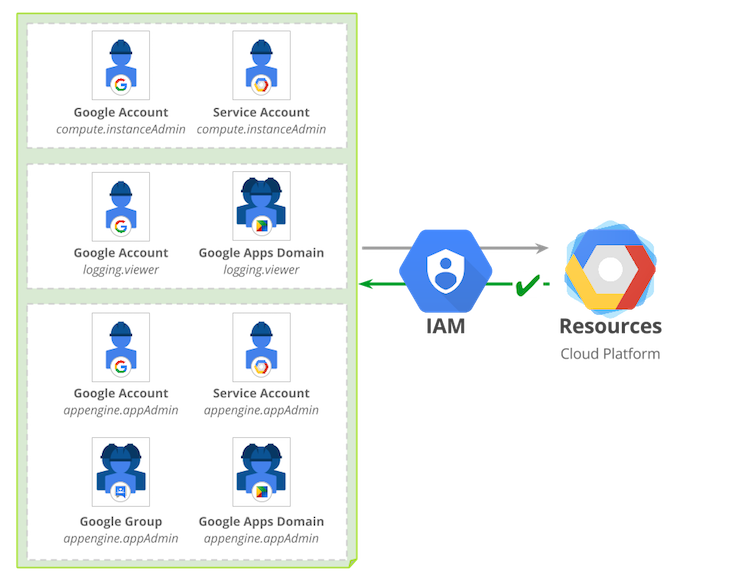
\includegraphics[width=0.5\textwidth]{./img/iampolicy.png} }%
	    	\subfloat[Cloud IAM Policy and Roles management]{ 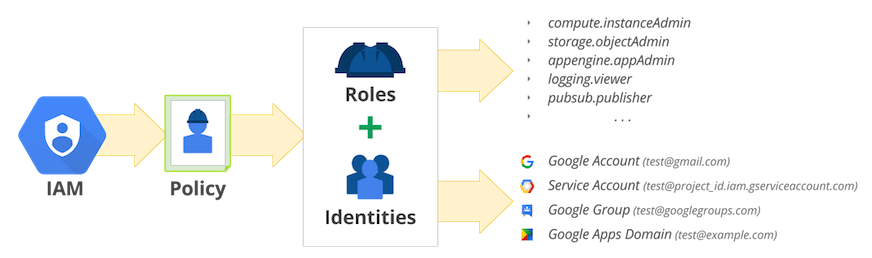
\includegraphics[width=0.8\textwidth]{./img/iam_overview.png} }%
    	
    \subfloat[Policy hierarchy]{ 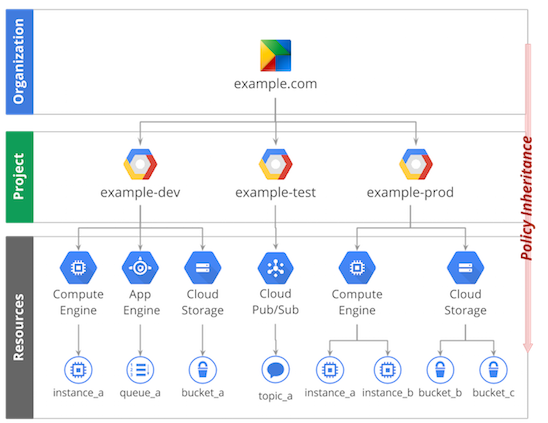
\includegraphics[width=0.7\textwidth]{./img/iampolicy-hierarchy.png} }%
	
    \caption[access]{Concepts of Cloud Identity and Access Management   \centering }
    \label{fig:iam}
\end{figure}


		\subsection{Cloud Storage}
		\label{subsub:datastore}
Google Cloud Storage allows storing data in a high level of availability and durability 
over the world. Storage of data is highly persistent by replication data over Google 
infrastructure. Service provide security protection based 
on model end-to-end, thus in-flight and at rest. For handling of data is available command 
line interface \textit{gsutil} and programming API for build 
reliable and fast networking application. The pricing model provides different tariffs 
according to data durability, availability and performance of storage.
        

\paragraph{Storage classes} are represented by three types of storage. The classification is based 
on a characteristic of storage. \textit{Standard storage}, offers high availability and low 
latency. This storage is suitable for frequent access such 
as data of web services or mobile applications.
Next class is \textit{Durable Reduced Availability} with less availability than  \textit{standard}. 
This class is suited for jobs, where unavailability is accepted or for a cost-sensitive project. 
Last class, \textit{Cloud Storage Nearline} is designed 
covered gap between mentioned classes. It provides slightly lower availability and slightly higher 
latency than Standard storage but for lower cost. 
Storage for data backup or archiving data is two explanation of use cases.

\paragraph{Buckets location} are configurable by three properties, specifically: global unique 
name, storage class and geographical location of where the bucket is stored.

\begin{footnotesize}
\begin{lstlisting}[style=mybash]
#creating two new buckets using command-line tool gsutil
$ gsutil mb -p my-project gs://mwdata gs://mwprocessed -c durable_reduced_availability
\end{lstlisting}
\end{footnotesize}
 

All buckets are covered under a single namespace thus, the name of bucket must be unique. 
Google defined rules for naming buckets which are based on DNS naming conventions. Validator 
during creation process responds error message in the wrong case. 

\paragraph{Objects} represents peace of data placed in storage. Object have two components: 
user data and metadata of quality. All \textit{objects} are immutable after creation. Thus 
incremental changes are not available. However, an object 
can be overwritten. Before the new version of an object is available, the old version is still 
reachable for reading. Overwriting of a single object 
can proceed up to one second. Otherwise \textit{503 Service Unavailable errors} is responded.

\paragraph{Consistency} of data are provided by global Google network of data centres. 
When success response is received, uploaded data are available from any location in 
Google network. Google has designed and constructed a private network 
for fast data transfer between their data centres around the word. Thus, data throughput 
of Google backbone network is higher than the capability of the 
internet-facing network. The latency for writing is slightly higher for replicated store 
than non-replicated. As an example of a strongly consistent behaviour 
is not accessible metadata of object immediately after deletion object. 
It is handled by \textit{404 Not Found} status code.


\subsubsection{Access control}
The configuration of access control can be set using \textit{gsutil} command-line tool 
or API. Cloud storage offers three different ways for access management for buckets and objects, which are described below.
\begin{itemize}
\item\textbf{Access Control lists (ACLs)} provide way manage read or write access for 
specified Google accounts and groups.
\item\textbf{Signed URLs (query string authentication)} provide a way to establish time 
limited read or write access to anyone who disposes of URL address. This way is a choice for users without Google account.   
\item\textbf{Signed Policy Documents} allows specifying what can be uploaded to a bucket. 
Size, content type and other specification can be set by policy handler. 
\end{itemize}
Additionally is available access control on the Project level. To control user's ability 
to access bucket on the project level is developed   \textit{Google Cloud Identity and Access Management}(IAM). This service is described on 
the and of the section.

\paragraph{Permissions} is logically divided to read, write and owner. For \textit{objects}, 
is available to let user download \textit{object} and modify metadata by owner. By 
default, \textit{objects} are owned by original requester who 
upload the \textit{object}. As \textit{object}, \textit{Buckets} are readable. In 
addition, list of user let them to create, overwrite and delete objects 
in \textit{bucket}. Owner can let user to read and write permission on the bucket 
include metadata. By default, \textit{buckets} are owned by the project 
owner group.

\paragraph{Scopes}\label{par:scopes}of authentication consists six methods for 
specifying ACL such as  Google Storage ID, Google account email address, Google 
group email address, Google Apps domain, Special identifier for all Google 
account holders and Special identifier for all users.

\begin{footnotesize}
\begin{lstlisting}[style=mybash]
#Identify an object that the user uploaded.
gsutil acl get gs://mwdata
\end{lstlisting}\end{footnotesize}
 

\paragraph{Access control list} is configurable by command line tools \textit{gsutil acl} 
or by API based on JSON or XML structures. The management of ACL is based on concentric 
permissions which provide faster configuration. When user grant 
write permission, automatically get also read permission. In case of grant of owner 
permission, read and write is also reachable. In addition, is available 
list of predefined ACL for quick settings of access restrictions such as project-private, 
private, public-read, public-read-write, authenticated-read, 
bucket-owner-read and bucket-owner-full-control.

\begin{footnotesize}
\begin{lstlisting}[style=mybash]
#usage of a predefined ACL to an object during object upload
gsutil cp -a bucket-owner-full-control mwbck.zip gs://mwdata
\end{lstlisting}
\end{footnotesize}
 


\subsubsection{Data control}
?

\paragraph{Accessing endpoints}
?

		\subsection{Networking}
		%https://cloud.google.com/compute/docs/networking#networks
%https://cloud.google.com/compute/docs/vm-ip-addresses
%%https://cloud.google.com/compute/docs/configure-instance-ip-addresses#internalstaticip
%https://cloud.google.com/sdk/gcloud/reference/compute/firewall-rules/create
%Rhttps://cloud.google.com/dataproc/cluster-web-interfaces


hive
https://cwiki.apache.org/confluence/display/Hive/Setting+Up+HiveServer2

		\subsection{Dataproc: Cluster services}
		\label{subsub:dataproc}
\textbf{Dataproc} is a package of tools for managing Hadoop\ref{sec:hadoop} 
and Spark\footnote{Apache spark: \url{http://spark.apache.org/}}.
The process of a deploying cluster is fully automatized using the default 
configuration. Hadoop and Spark deployment are compatible with official
releases. By default, the configuration of automatic deployment is simple. 
On the other hand in the most cases, it is 
necessary to configure cluster manually to fulfil custom requirements. 
Next to standard command-line tool \textit{gcloud} for handling deployment is 
helper software \emph{bdutil} for deploying cluster allows complex 
configuration includes 
defining hardware configuration, combining services from wide Google cloud 
portfolio and custom additional tasks for installation and configuration cluster. 
This command-line utility are based on authentication provide by \textit{gcloud} interface.

In the list of the main characteristic of \textit{Dataproc} solution is a 
low cost, quick starting and integration with Google Cloud services. 
The pricing is  \$0.01 per CPU for an hour(19.3.2016). Dataproc service can 
include \textit{Preemptible instances} which offers pricing 
per minutes(min 10 minutes). This choice is suitable for batch jobs and 
fault-tolerant workloads. The time for starting cluster is up to 
90 seconds in average. To compare e.g with Amazon cloud services(EMR)\cite{amazon_emr}, 
starting Google cluster is 3 times faster.

\paragraph{Create and manage cluster} Deploying process can be handled by three main 
ways. First, using \textit{gcloud} command-line tool. Second, by running \textit{bdutil}\ref{subsub:bdutil} 
script and the last option, with using 
\textit{Cloud Dataproc API} - \textit{cluster.create}. Google Cloud web interface offers 
framework for cluster deployment as well, but the configuration and 
management is considerably limited. 
Command-line tool \textit{gcloud} consist parameters: \textit{cluster} for managing and 
describing cluster, \textit{jobs} for submitting 
and managing jobs on cluster, finally parameter \textit{operation} for handling operation, 
like cancel or delete active
 operation by \emph{operation\_id}. For more advanced cluster deployment is suited script 
 tool \textit{bdutil} which is 
 package for custom configuration of cluster. The advantages is easy redeployment and 
 reproducibility custom
  configuration of cluster. 



\begin{footnotesize}
\begin{lstlisting}[style=mybash]
#creation of cluster with default settings using command-line tool gcloud
$ gcloud dataproc clusters create <cluster-name>
\end{lstlisting}
\end{footnotesize}
 

\paragraph{Cluster Properties} are by default configured to deploy cluster with desired 
number of nodes. The configuration behind is not trivial but Google \textit{Dataproc} provide 
automatic deployment without big investments. The 
configuration of open source software as Spark, Hadoop  and extensions as Hive are based 
on several XML and plain text configuration files. For cluster deployment 
using \textit{Dataproc}, the configuration is based on the same configuration files.Some 
properties are reserved by Google and cannot be overridden 
to protect functionality of Cloud Dataproc. The crucial feature of cluster is immutable 
configuration after start. Thus, all configuration must be set 
properly before starts of daemons on cluster. For apply changes must be cluster redeployed. 

\paragraph{File system}
Google Cloud Dataproc offers two different storages based on distributed file systems. In 
chapter Hadoop\ref{subsec:hdfs} is described Hadoop Distributed File system(HDFS) which is 
default file system for Apache Hadoop framework and is as optional in Google Services. As 
default file system for Hadoop and Spark deployment provided by Google Cloud is \textit{Google Cloud storage}. 

Google Claude Storage offers direct data access in available storage for the rest of Google 
services. In addition the interoperability provide access between Spark and Hadoop on Google. 
Next advantage is high data availability provided by Cloud
 Storages, with high availability and global replication without less performance. The key 
 feature is data access after cluster is shouted down. The 
pricing of cluster instance is based on time. Thus, to save costs, cluster should run only when 
is used. With using HDFS as distributed file system, after 
shutting down cluster instance, data are removed and lost as well. In contrast, data stored on 
Claude Storage are available after cluster is stopped and 
can be linked again in further cluster deployment.

Interaction between Hadoop Distributed System and Dataproc cloud is limited to compare default 
Google Storage. HDFS is scalable across VM’s, but doesn’t scale per instance as well as Claude Storage due to VM disk bandwidth limits. 

\paragraph{Machine type} Google Cloud Datagram clusters are built on Google Compute Engine instances.
\textit{Machine types} configuration define the virtualized hardware resources available to an 
virtual machine instance. Two ways how to define configuration are available: \textit{predefined instance} and \textit{custom machine types}.  

\begin{footnotesize}
\begin{lstlisting}[style=mybash]
# print list of predefined instances
$ gcloud compute machine-types list
NAME           ZONE           CPUS MEMORY_GB DEPRECATED
f1-micro       asia-east1-c   1     0.60
g1-small       asia-east1-c   1     1.70
n1-highcpu-16  asia-east1-c   16   14.40
...
\end{lstlisting}
\end{footnotesize}


Customization of machines availability is suitable for project with workloads where the computing 
engine require high performance machine resources or just where predefined machines are not a good 
fit to workloads. Once a custom machine template is 
defined, the configuration is available for all connected services over Google Claude portfolio.

\subsubsection{bdutil: Spark and Hadoop on Google Cloud}\label{subsub:bdutil}
As has been already mentioned, \textit{bdutil} is a command line script designed for
managing Hadoop instance on Google Compute Engine. It provide deployment, configuration
and shut-down Hadoop instances in quickly and reproducible way, even for complex configuration. 
Script is based on Bash v3 or later which is available on VM of Google Compute Engine or most of 
Linux distributions. In addition to shell command-line
tools \textit{gcloud dataproc}, \textit{bdutil} includes configurable scripts for deployment 
Spark and Hadoop. The default configuration is Hadoop 1 with Cloud Storage as the storage system. 
Furthermore, \textit{bdutil} is designed to allow writing custom environment variable configuration 
files. For example: \emph{CONFIGBUCKET} - path to Google Storage, \emph{PROJECT} - ID of Google Platform 
project or \emph{GCE\_MACHINE\_TYPE} - machine type of the Google Compute Engine.

	
    
\section{Related Technologies Behind}
    \subsection{Geospatial framework GRASS GIS}

\textit{"\textbf{Geographic Resources Analysis Support System}, 
commonly referred to as GRASS GIS, is a Geographic Information System (GIS) used for
 data management, image processing, graphics production, 
spatial modelling, and visualization of many types of data. It is Free (Libre) Software/Open
 Source released under GNU General Public License 
(GPL) >= V2. GRASS GIS is an official project of the Open Source Geospatial Foundation."\footnote{Cited from:
 \url{https://grass.osgeo.org/documentation/general-overview/}}}

 \begin{figure}[!htbp]
    \centering
    
\includegraphics[width=0.2\textwidth]{./img/grasslogo.png}
    \caption[Logo GRASS]{\centering Logo of GRASS GIS.}
 \end{figure}   
GRASS GIS vector map is a data layer which consists number set of a feature in geographic space. 
These objects are represented by points, lines, polygons, and volumes. Usually, each feature in the 
map is somehow connected with the set of attribute \textit{layers} stored in a database. 

In GRASS GIS is a available driver which allows using several database backends for manipulation 
with vector data. The main module for import and export of vectors datasets is v.in.ogr and v.out.ogr 
which is based on widely used GDAL library. 
In the current stable version of GRASS GIS is implemented a driver for PostGIS support. PostGIS is 
an extension of object-rational PosgreSQL database which brings the support for geographic objects. 
In addition PostGIS extension consist package of 
location-based function for building a spatial query. Such an ESRI Spatial Framework for Hadoop 
brings the support of spatial analysis for HIVE analogically PostGIS 
already have been developed as a spatial extension for PostgreSQL.  

The key feature for this project is the fact that GDAL OGR supports GeoJSON data format, which is suitable 
for storing and analysing data using MapReduce framework. The description of GeoJSON and its serialization is 
mandatory due to the design of MapReduce 
for parallel computing. GeoJSON and its features are described in the second part of the work\ref{json}.

\paragraph{Vector data}


GRASS vectors 
%can be linked to one or many database management systems (DBMS). The db.* set of commands provides 
%basic SQL support for attribute management while the v.db.* set of commands operates on a table 
%linked to a vector map. Import and export of vector data are handled with v.in.ogr module. The 
%v.in.ogr module offers a common interface for many different vector formats. For special cases, 
%other import modules are available, e.g. v.in.ascii for input from a text file containing coordinate 
%and attribute data, and v.in.db for input from a database containing coordinate and attribute data. 
%With v.external external maps can be virtually linked into a mapset, only pseudo-topology is generated 
%but the vector geometry is not imported. The v.out.* set of commands exports to various formats. 
%GRASS 7 allows accessing PostGIS data directly via virtual mapset called OGR. In this case parameter, 
%map or input is used for OGR data source and layer for a table.


    \subsection{Apache Hive }
\textit{\footnote{Cited from: \url{https://hive.apache.org/}}"The Apache Hive ™ data warehouse software 
facilitates querying and managing large datasets residing in distributed storage. Hive provides a mechanism 
to project structure onto this data and query the data using an SQL-like language called HiveQL. At the same
time, this language also allows traditional map/reduce programmers to plug in their custom mappers and 
reducers when it is inconvenient or inefficient to express this logic in HiveQL."}


%%%%%%%%%%%%%%%%%%%%%%%%%%%%%%%%%%%%%%%%%%%%%%%%%%%%%%%%%%%%%%%%%%%%%%%%%%%%%%%%%%%%%%%%%%%%%%%%%%%%%%%%%%%%%%%%%%%%%%%%%%%
%%%%%%%%%%%%%%%%%%%%%%%%%%%%%%%%%%%%%%%%%%%%%%%%%%%%%%%%%%%%%%%%%%%%%%%%%%%%%%%%%%%%%%%%%%%%%%%%%%%%%%%%%%%%%%%%%%%%%%%%%%%
%%%%%%%%%%%%%%%%%%%%%%%%%%%%%%%%%%%%%%%%%%%%%%%%%%%%%%%%%%%%%%%%%%%%%%%%%%%%%%%%%%%%%%%%%%%%%%%%%%%%%%%%%%%%%%%%%%%%%%%%%%%
%%%%%%%%%%%%%%%%%%%%%%%%%%%%%%%%%%%%%%%%%%%%%%%%%%%%%%%%%%%%%%%%%%%%%%%%%%%%%%%%%%%%%%%%%%%%%%%%%%%%%%%%%%%%%%%%%%%%%%%%%%%

\newpage
\chapter*{Experiment framework}\stepcounter{chapter}\addcontentsline{toc}{chapter}{Practical framework}
\paragraph{Goals}


\section{Setup working environment}
As the main resource of data storage and computing engine for practical framework has been used Google Cloud Platform.
 Thus, all configuration of Hadoop cluster, data storage, and networking is linked to cloud services. Additionally,
  development of GRASS client framework for Hadoop and consequential testing  as well.

Google Cloud Platform offers free trial 60 days promotion for using their services. The offer is limited by two
 months or 300 \$ for whichever services of Google Cloud portfolio.
        \subsection{Set up project: gcloud}
Using Google Cloud Platform web interface has been created new project placed in App Engine 
location \textit{europe-west}. The project is characterized by Project name, Project ID and billing account.
On local computer has been installed Cloud SDK which includes \textit{gcloud} 
and \textit{gsutil} tools for remote control Google Cloud services.
Initialization of gcloud using command \emph{gcloud init}\footnote{To initialize project on remote computer 
without X Window System forwarding must be used flag \emph{--console-only}.} provide authentication process using web browser 
and request of access to the project.

Compute Engine uses a default zone and region based on information from the project metadata. In this case, 
configuration has been inherited from the Project settings without an additional configuration.


\subsection{Data management}
        Google Data Store is used as the main data house for project. Command line tool \textit{gsutil} 
        allows object operations stored in buckets of Google. For copying large object is very suitable to use 
        a function for slicing which allows parallel 
        downloading and uploading.
        
For downloading object using HTTP request gsutil perform slicing object on Google Storage  and preallocate 
space in the destination folder. The final file is renamed after all slices are processed. For downloading 
is not required additional space on local disk. 
The performing of slices is configurable by parameter \textit{sliced\_object\_download\_threshold} which 
define a maximum number of slices. It can be 
useful to protect the disk from overloading. For efficient uploading of large files is crcmod which required 
an installation  of CRC32C package. 

\paragraph{SQL data migration} Within project have been created several buckets for storing exported 
data from SQL. Data captured by microwave operator T-Mobile has been described in my bachelor theses\cite{bp_krejci}. 
Date are stored in relation database 
PostgreSQL and includes over $3e9$ rows. Due to big data characteristic has been developed python\ref{py:export} 
script for exporting data in defined time 
interval. It protects a database from overloading by queries for all rows in one query. 

As a machine for exporting, merging and uploading data to bucket was used VM instance from Google Compute engine.

\begin{footnotesize}
\begin{lstlisting}[style=mybash]
#create compute engine with 500 GB persistent disk
$ gcloud compute --project "spatial-hadoop" disks create "vmexport" --size "500" \
--zone "europe-west1-b" --type "pd-standard" --image \
"/debian-cloud/backports-debian-7-wheezy-v20160418"
\end{lstlisting}
\end{footnotesize}
 
Table public.record from mwdb database has been exported in time step one week. The merge of each exported 
csv files has been merged using Unix \textit{cat} command. The size of exported table record is around 98 GB or 17 GB tarball.


\begin{footnotesize}
\begin{lstlisting}[style=mybash]
#create bucket 
$ gsutil mb -l EU gs://mwdata_export
#copy big file with slicing
$ gsutil -m -o GSUtil:parallel_composite_upload_threshold=100M cp \
mwdump.csv gs://mwdata_export/
\end{lstlisting}
\end{footnotesize}
 
\subsection{Networking}
https://dzone.com/articles/hadoop-rest-api-webhdfs



        \subsection{Hadoop deployment}
        
For deployment of Hadoop cluster is used bdutil command line package builds from several bash scripts 
and XML configuration files of Hadoop and its extensions. In the section below is described a essential 
configuration of Hadoop on Google Dataporoc 
service. Mainly is shown the important part which touches requirements for using Esri spatial frameworks for Hadoop. 

Google Claude Dataproc brings to the cloud field automated deployment of Hadoop cluster. To compare 
with manual configuration of Hadoop cluster, it allows fast and efficient deployment without spending 
extra time mainly on network configuration.

The configuration files for \textit{'standard'} Hadoop are stored in \textbf{\$HADOOP\_HOME\\/conf/} 
and consist  primary xml files. Many of parameters are defined by default and they may be omitted in configuration files. In addition, the default 
configuration folder  includes shell file which specified environment variables of Hadoop Daemon. Default configuration folder lists:
\begin{itemize}
\item \textbf{hadoop-env.sh} The file specifies environment variables that affect JDK used by daemons
for example \textbf{\$JAVA\_HOME}.
\item \textbf{core-site.sh}   This file informs Hadoop deamon where namenode runs in the cluster. Furthermore 
information about port number used for Hadoop instance, memory limit for data size,  memory allocated for HDFS, and size of read and write buffers.
\item \textbf{hdfs-site.sh}  This file contains the configuration settings for HDFS daemons, the Name 
Node, the Secondary Name Node, and the data nodes. Usually is configured block replication and permission checking on HDFS. 
\item \textbf{mapred-site.sh}  This file contains the configuration settings for MapReduce daemons 
such the JobTracker and the TaskTracker.
\end{itemize}

in addition default configuration directory includes two flat files: \textit{masters} and \textit{slaves}. 
Both includes hostname of slaves or master where each line represents one address. 
Master file informs about the Secondary Namenode location to Hadoop daemon. The \textit{masters} 
file at Master server contains an IP address of Secondary Name Node servers.
The second one, \textit{slaves} on Slave server contains the IP address of the slave node. Notice 
that the \textit{slaves} file at Slave node contains only its own IP address and not of any other Data Nodes in the cluster.


\paragraph{Hadoop modes} characterize cluster features of Hadoop and its distributed file system. 
There are main three approaches of cluster mode which are described below:
\begin{itemize}
\item \textbf{Standalone mode} If Hadoop is installed on a machine, by default is preconfigured to a 
non-distributed mode as a single Java process. This mode  is suitable for MapReduce development and debugging.
\item \textbf{Pseudo-Distributed mode}  configuration allows to run  Hadoop on single-node and behave
 like multi-node. It's provided by running Hadoop daemons in separate Java processes. To configure pseudo-distributed Hadoop must be modify \textit{core-site.xml} and \textit{hdfs-site.xml} file\cite{hadoop_modes}.  


\begin{footnotesize}
\begin{lstlisting}[style=python]
#etc/hadoop/core-site.xml:
-
<configuration>
    <property>
        <name>fs.defaultFS</name>
        <value>hdfs://localhost:9000</value>
    </property>
</configuration>


#etc/hadoop/hdfs-site.xml: 
-
<configuration>
    <property>
        <name>dfs.replication</name>
        <value>1</value>
    </property>
</configuration>
\end{lstlisting}
\end{footnotesize}

\item \textbf{Fully distributed cluster} is an ideal approach for harnessing the potential of
 parallel computations. The nodes are on virtualized machines with assigned machine capability 
 such a CPU, memory, and disk. The most efficient approach which is used in the production or 
 in large clusters is an installation of Hadoop directly on the machine with Linux without virtualised environment.

\end{itemize}


\subsubsection{Configuration}
In contrast to standard Hadoop deployment, a configuration in \textit{Dataproc} using bdutil is 
extended by parameters and configuration files which handle automated deployment and other Google
Cloud Services. The files in bdutil can be divided into two groups. In the first,  are shell scripts 
which can be run during cluster deployment.

Tool bdutil comes with several bash scripts which set essentials characteristic of the cluster 
such as a type of framework- Hadoop or Spark, version of Hadoop, Hadoop extension(HIVE,PIG), 
connectors to other services of Google etc.


% Please add the following required packages to your document preamble:
% \usepackage{booktabs}
\begin{table}[!htbp]
\begin{scriptsize}
\centering
\begin{tabular}{@{}|l|l|@{}}
\toprule
Bash script                              & Description                                                                                                                                              \\ \midrule  \midrule
bdutil\_env.sh                           & The base of configuration. It is always run by bdutil. Must be modified \ref{bdutilenv}                                                                                  \\ \midrule
single\_node\_env.sh                     & \begin{tabular}[c]{@{}l@{}}Deploys a pseudo-distributed cluster on a single VM. \\ This approach is suitable for testing clients etc.\end{tabular}       \\ \midrule
hadoop2\_env.sh                          & \begin{tabular}[c]{@{}l@{}}Deploys a cluster with the latest stable version of  Hadoop 2.x  \\instead of the traditional Hadoop 1.x version.\end{tabular} \\ \midrule
bigquery\_env.sh                         & \begin{tabular}[c]{@{}l@{}}Deploys a cluster with the BigQuery connector for  Hadoop installed.\\ Not compatible with hadoop2\_env.sh.\end{tabular}      \\ \midrule
extensions/querytools/querytools\_env.sh & \begin{tabular}[c]{@{}l@{}}Deploys a cluster with Apache Pig and Apache Hive installed. \\ Not compatible with hadoop2\_env.sh.\end{tabular}             \\ \midrule
extensions/spark/spark\_env.sh           & Deploys a cluster with Apache Spark installed.                                                                                                           \\ \bottomrule
\end{tabular}
\caption{Configuration bash scripts of bdutil \cite{gc_hadoop}}
\label{bdutil:configsh}
\end{scriptsize}
\end{table}



\begin{table}[!htbp]
\centering
\begin{scriptsize}
\begin{tabular}{@{}lll@{}}
\toprule
\multicolumn{1}{|l|}{File}                        & \multicolumn{1}{l|}{Name}                         & \multicolumn{1}{l|}{Value}              \\ \midrule \midrule
\multicolumn{1}{|l|}{\multirow{17}{*}{bdutil\_env.sh}} & \multicolumn{1}{l|}{CONFIGBUCKET}                 & \multicolumn{1}{l|}{mwdata\_export}     \\ \cmidrule(l){2-3} 
\multicolumn{1}{|l|}{}                                 & \multicolumn{1}{l|}{PROJECT}                      & \multicolumn{1}{l|}{spatial-hadoop}     \\ \cmidrule(l){2-3} 
\multicolumn{1}{|l|}{}                                 & \multicolumn{1}{l|}{GCE\_IMAGE}                   & \multicolumn{1}{l|}{debian-7-backports} \\ \cmidrule(l){2-3} 
\multicolumn{1}{|l|}{}                                 & \multicolumn{1}{l|}{GCE\_MACHINE\_TYPE}           & \multicolumn{1}{l|}{n1-standard-2}      \\ \cmidrule(l){2-3} 
\multicolumn{1}{|l|}{}                                 & \multicolumn{1}{l|}{GCE\_ZONE}                    & \multicolumn{1}{l|}{europe-west1-b}     \\ \cmidrule(l){2-3} 
\multicolumn{1}{|l|}{}                                 & \multicolumn{1}{l|}{GCE\_NETWORK}                 & \multicolumn{1}{l|}{default}            \\ \cmidrule(l){2-3} 
\multicolumn{1}{|l|}{}                                 & \multicolumn{1}{l|}{GCE\_MASTER\_MACHINE\_TYPE}   & \multicolumn{1}{l|}{n1-standard-4}      \\ \cmidrule(l){2-3} 
\multicolumn{1}{|l|}{}                                 & \multicolumn{1}{l|}{PREEMPTIBLE\_FRACTION}        & \multicolumn{1}{l|}{1.0}                \\ \cmidrule(l){2-3} 
\multicolumn{1}{|l|}{}                                 & \multicolumn{1}{l|}{PREFIX}                       & \multicolumn{1}{l|}{hadoop}             \\ \cmidrule(l){2-3} 
\multicolumn{1}{|l|}{}                                 & \multicolumn{1}{l|}{NUM\_WORKERS}                 & \multicolumn{1}{l|}{2}                  \\ \cmidrule(l){2-3} 
\multicolumn{1}{|l|}{}                                 & \multicolumn{1}{l|}{MASTER\_BOOT\_DISK\_SIZE\_GB} & \multicolumn{1}{l|}{200}                \\ \cmidrule(l){2-3} 
\multicolumn{1}{|l|}{}                                 & \multicolumn{1}{l|}{DEFAULT\_FS}                  & \multicolumn{1}{l|}{gs}                 \\ \cmidrule(l){2-3} 
\multicolumn{1}{|l|}{}                                 & \multicolumn{1}{l|}{ENABLE\_HDFS}                 & \multicolumn{1}{l|}{false}              \\ \cmidrule(l){2-3} 
\multicolumn{1}{|l|}{}                                 & \multicolumn{1}{l|}{ENABLE\_HDFS\_PERMISSIONS}    & \multicolumn{1}{l|}{false}              \\ \cmidrule(l){2-3} 
\multicolumn{1}{|l|}{}                                 & \multicolumn{1}{l|}{INSTALL\_GCS\_CONNECTOR}      & \multicolumn{1}{l|}{true}               \\ \cmidrule(l){2-3} 
\multicolumn{1}{|l|}{}                                 & \multicolumn{1}{l|}{CORES\_PER\_MAP\_TASK}        & \multicolumn{1}{l|}{1.0}                \\ \cmidrule(l){2-3} 
\multicolumn{1}{|l|}{}                                 & \multicolumn{1}{l|}{CORES\_PER\_REDUCE\_TASK}     & \multicolumn{1}{l|}{1.0}                \\ \midrule
\multicolumn{1}{|l|}{hdfs-template.xml}                & \multicolumn{1}{l|}{dfs.webhdfs.enabled}          & \multicolumn{1}{l|}{true}               \\ \midrule

\end{tabular}
\caption{Selected configuration parameters of bdutil tool}
\label{bdutil:config.sh}
\end{scriptsize}
\end{table}
\paragraph{bduitl\_env.sh}\label{bdutilenv}The main script called \textit{bdutil\_env.sh} consists mandatory 
and free environmental variables for setting environment, hardware and deployment configuration.

\begin{itemize}
\item \textbf{Environment variables} provide the setting which refers to the id of the project and to 
the default bucket in GCS. The defined bucket holds SSH keys and configuration of the file system. In 
the case of usage GCS as a file system for Hadoop, the defined GCS is linked  during cluster deployment 
and all files are natively accessible by standard Hadoop commands e.g copy file \textit{hadoop fs -cp  /data/* /tmp/}.

\item \textbf{Hardware configuration}
allows to specify name, shape, location and size of a cluster. As important can be a definition of machine
 type, with reflecting final performance of cluster and pricing of service as well. In addition, the parameter 
 for a number of workers and size of the disk are also crucial.

Hardware configuration allows setting different disk size and  disk type to master and workers. Furthermore, 
extra persistent disks(PDs) can be listed. Available virtual machines of service account can be attached to a 
further cluster. For that case, the GCS connector must by allowed.

\item \textbf{Deployment} section consist parameters for customizing Hadoop installation on VMs workers 
and master. The configuration of GCS connector allows to use as a distributed file system \textit{GS} and 
\textit{BIGQUERRY} connector allows read/write access to Google BigQuery. File system of a cluster is set 
by default to gs(google storage), the second 
option is standard HDFS. This group consists several path configuration for defining the destination of 
Hadoop installation and its related files. Furthermore is essential to configure permission  of \textit{HDFS} data access.

Parameter CORES\_PER\_MAP\_TASK and CORES\_PER\_REDUCE\_TASK must be defined as a decimal number which 
controls the number of maps and reduces slots on each node.The number is computed as a ratio of the 
number of virtual cores on the node. For example if the machine of specification \textit{ n1-standard-2} 
is used(2 cores) and the parameter is set to 1 would have $\dfrac{2}{1} = 2$ map/reduce slots.
\end{itemize}


\paragraph{Hadoop configuration} files  are stored in \textit{conf/hadoop1} for Hadoop version 1.x VM and 
\textit{conf/hadoop2} for 2.x version both are placed within \textit{bdutil} base directory. In compassion 
to standard Hadoop configuration files, these are extended by files for configuration Bigtable(Hadoop1.x), 
BigQuery(Hadoop2.x) and GCS. Particular values of parameters are linked over environment variables to  to 
the main script \textit{bdutil\_env.sh} and other bash files stored in directory \textit{libexec}. In 
example below is shown configuration of task tracker where the value is set by global variable 
\textit{MAP\_SLOTS}. To call global variable must be used convention \textit{envVar name=""}.

\begin{footnotesize}
\begin{lstlisting}[style=XML]
<?xml version="1.0" encoding="UTF-8"?>
<?xml-stylesheet type="text/xsl" href="configuration.xsl"?>
<configuration>
   <property>
      <name>mapred.tasktracker.map.tasks.maximum</name>
      <value><envVar name="MAP_SLOTS" /></value>
      <description>The maximum number of map tasks that will 
    be run simultaneously by a tasktracker.</description>
   </property>
</configuration>
\end{lstlisting}
\end{footnotesize}


 
As mentioned, in Dataproc are available two version of Hadoop. For two spatial frameworks as from 
ESRI and HadoopGIS must be used version 1.x of Hadoop due to dependency on Hive, which is in Google 
Dataproc incompatible with versions Hadoop 2.x. The main limitation of the versions 1.x is unsupported 
YARN framework which is the next generation of MapReduce framework also called MapReduce 2.0 (MRv2)\cite{yarn}. 
The main difference between is the architecture where JobTracker, resource management, and job scheduling are split into separated daemons.


Modification properties during run https://cloud.google.com/dataproc/concepts/cluster-properties
	

\paragraph{Running cluster} is done by executing bdutil bash file with flags and parameters.  
Flag \textit{--env\_var\_files} run selected bash files from the predefined group \ref{bdutil:configsh}. 
Besides predefined bash files is possible to add a custom script which be executed as well. The  order 
of files execution is according to the sort in the list. The main script \textit{bduitl\_env.sh} 
\ref{bdutilenv} is executed as default first without presence in the list. Below is in the list script 
for downloading and compiling spatial frameworks for Hadoop and their dependency. Bash script \textit{spatial.sh} shown below 
%
\begin{footnotesize}
\begin{lstlisting}[style=python]
COMMAND_GROUPS+=(
  'install_spatial:
     spatial1.sh
  '
)

COMMAND_STEPS+=(
  'install_spatial'
)
\end{lstlisting}
\end{footnotesize}
is defined by command group where is defined a path to the bash for execution. List of command steps is a
 global variable and its items appends to execution the list.
 !!!!Staging binaries
 
 \begin{footnotesize}
\begin{lstlisting}[style=python]
ROLE=$(/usr/share/google/get_metadata_value attributes/role)
if [[ "${ROLE}" == 'Master' ]]; then 
	do----
fi
\end{lstlisting}
\end{footnotesize}
 
\$ gcloud dataproc clusters create my-dataproc-cluster \
    --initialization-actions gs://my-bucket/download-job-jar.sh
 
 
 
\begin{itemize}
\item \textbf{Case 1 - development configuration}  This configuration of cluster suits well to debugging 
of Hadoop and Hive client site. Cluster is configured as pseudo mode.
\begin{footnotesize}
\begin{lstlisting}[style=python]
$ ./bdutil -P spatial-cluster --env_var_files \
extensions/querytools/querytools_env.sh,single_node_env.sh,spatial.sh deploy
\end{lstlisting}
\end{footnotesize}


\item \textbf{Case 2 - computational configuration}  To compare configuration above, Case 2 is fully 
distributed deployment of cluster. To modify temporally settings of hardware, storage etc. can be used 
additional reconfiguration using flags, which overwrite default one.
%
\begin{footnotesize}
\begin{lstlisting}[style=python]
$ ./bdutil -P spatial-cluster --num_workers 10 \
     --machine_type n1-standard-6\
     --env_var_files \
     extensions/querytools/querytools_env.sh,spatial.sh deploy
\end{lstlisting}
\end{footnotesize}

\end{itemize}


%# Set the default filesystem to be 'hdfs' since Pig and Hive will tend to rely
%# on multi-stage pipelines more heavily than plain Hadoop MapReduce, and thus
%# be vulnerable to eventual list consistency. Okay to read initially from GCS
%# using explicit gs:// URIs and likewise to write the final output to GCS,
%# letting any intermediate cross-stage items get stored in HDFS temporarily.
%DEFAULT_FS='gs'




            \subsubsection{Scaling cluster}
            \subsubsection{Logging}
 
 
 
        
\section{GRASS Hadoop framework}
\paragraph{Background}
Desktop application GRASS GIS became as a powerful environment for analysing spatial data, which can 
reach characteristic of big data. In a box of GRASS GIS are thousands of modules   The main motivation 
behind GRASS GIS framework for Hadoop is a vision to allow user to process processing big data natively from desktop environment. In proprietary GIS field, ESRI comes with package \textit{Geoprocessing tools for Hadoop}\cite{esri_gtfp} 
which has been implemented for ArcMap desktop application as a native interface for interaction with 
their Java library \textit{Esri Spatial framework for Hadoop}. More specifically, the tools enable:

\begin{itemize}
\item exchange data between ArcGIS Geodatabase and a Hadoop system, and allows ArcGIS to run Hadoop workflows jobs,
\item copy data files from ArcGIS to Hadoop, and copy files from Hadoop to ArcGIS, and 
\item run an Oozie workflow in Hadoop, and to check the status of a submitted workflow.
\end{itemize}
 
 
In first the chapter\ref{summary_libs} of theses has been described and summarized features of three different frameworks for processing large scale data. 
As the most suitable framework for the this project became Esri framework, which can be deployed without extra customisation, natively includes considerable package of spatial functions, furthermore the documentation  and examples of usage are  the most comprehensive. Selected library has been used for testing and for explanation of usage. On the other hand although other libraries have not been tested, the modular design of framework allows to partition each steps of process which ensure easier future development with another aim. For example, user can generate GeoJSON from GRASS map and load it  to HDFS using \textit{hdfs.import.vector}, after that, create Hive table using \textit{hive.json.table} and load data. These steps are independent on any spatial library. Thus the interface for interaction between GRASS and Hive/Hadoop can be used as library for future development of another project. Currently, the framework supports HadoopGIS as well but the testing is not provided within this work.
 

  \begin{figure}[!htbp]
    \centering
    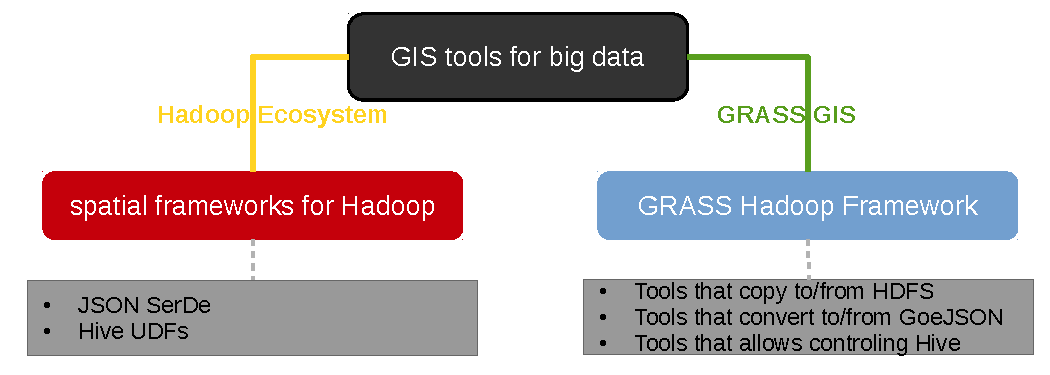
\includegraphics[width=1\textwidth]{./img/idea_schema.pdf}
    \caption[Resources]{\centering Resources for processing big data within desktop GIS}
 \end{figure} 

				
\subsection{Functionality}
The GRASS Hadoop Framework(GHF) can be described as Add-ons package of modules for GRASS GIS which supports interaction between GIS desktop environment and Hadoop/Hive. Although GHF can be used for transferring data between file system and HDFS. The main purpose is to bring possibility of usage of spatial frameworks developed for Hadoop to the GIS desktop application. 

Hadoop based spatial library for data processing can be used externally from the command line console e.g. \textit{hiveserver2} console or \textit{hadoop fs} tool. This approach can be more powerful for experienced users whit administration access to the cluster and knowledges of scripting, best in bash. If we assume that average user prefer friendly interface, than GHF is suitable choice. 

The package includes several modules\ref{tbl:modules} for managing connections, exporting GRASS maps to customised GeoJson(suitable for serialisation), loading them to HDFS, creating tables in Hive, loading data into table and after processing, importing result back to GRASS.


\begin{table}[!htbp]
\centering
\begin{scriptsize}
\begin{tabular}{@{}|l|l||l|l|@{}}
\toprule
hdfs.* modules  & description                    & hive.* modules  & description               \\ \midrule \midrule
hdfs.db.connect & Management of connections      & hive.json.table & Create table for GeoJSON  \\ \midrule
hdfs.in.fs      & Put data to HDFS from local       & hive.csv.table  & Create table for csv data \\ \midrule
hdfs.in.vector  & Put GRASS vectors to HDFS      & hive.execute    & Execute Hive command      \\ \midrule
hdfs.out.vector & Put vectors from HDFS to GRASS & hive.select     & Execute Hive query        \\ \midrule
hdfs.info       & HDFS metadata                  & hive.info       & Hive metadata             \\ \bottomrule
\end{tabular}%
\end{scriptsize}
\caption{Modules of GRASS Hadoop Framework}
\label{tbl:modules}
\end{table}



\subsubsection{Connection management} 
The handler of connection drivers for Hadoop and Hive is covered under \textit{hdfs.db.connect}. The module allows to hold connection profiles in default GRASS GIS database backend which is  by default SQLite database. The design of usage of database manager is derived from current GRASS db.* modules. Thus based on setting primary connection which is use for all interaction between database and GRASS. In contrast, database manager for HDFS allows to set connection id and its driver. Thus for each type of database(driver) can be stored several user connections distinct by user defined id(\textit{conn\_ide} parameter) and each driver can has only one primary connection.

\begin{table}[!htbp]
\begin{scriptsize}
\centering
\begin{tabular}{@{}|l|l||l|l|@{}}
\toprule
parameters    & description                                                                                               & flags & description                                                                             \\ \midrule \midrule \midrule
driver        & \begin{tabular}[c]{@{}l@{}}Type of database driver.\\ options: \\ hiveserver2, hdfs, webhdfs\end{tabular} & -c    & Print table of connection                                                               \\ \midrule
conn\_id      & identificator of connection                                                                               & -p    & Print active connection                                                                  \\ \midrule
host          & connection host                                                                                           & -r    & Remove all connections                                                                  \\ \midrule
port          & port of database                                                                                          & -t    & Test connection by conn\_type                                                           \\ \midrule
login         & user login                                                                                                & -a    & \begin{tabular}[c]{@{}l@{}}Set active connection\\  by conn\_id and driver\end{tabular} \\ \midrule
passwd        & password to database                                                                                      & --h   & Print usage summary                                                                     \\ \midrule
schema        & set active schema in db.                                                                                  & --v   & Verbose module output                                                                   \\ \midrule
authmechanism & support PLAIN mechanism                                                                                   & --q   & Quiet module output                                                                     \\ \midrule
connectionuri & connection uri of database                                                                                & --ui  & Force launching GUI dialog                                                              \\ \midrule
rmi           & Remove connection by id                                                                                   &       &                                                                                         \\ \bottomrule
\end{tabular}
\caption{Flags and parameters of \textit{hdfs.db.connection} module.}
\label{tbl:connections}
\end{scriptsize}
\end{table}

\paragraph{Defining connection} Parameter \textit{driver} and \textit{conn\_id} are mandatory for any connection profile. Parameter \textit{driver} define the protocol for communication with database and  and \textit{conn\_id} is a free unique string of connection profile. Other parameters as \textit{host}, \textit{port}, \textit{login}, \textit{passwd}, \textit{schema}, \textit{authmechanism} depends on a configuration of database server. After new connection is added, the module automatically set the new one as active. 

\paragraph{Connections management} Module offers several flags for handling management of connections. In table\ref{tbl:connections} are described flags and theirs functions. In case of controlling several Hadoop clusters is suitable  approach to define its connection profiles  and switching between by setting the primary one by flag -a with parameter \textit{conn\_id} and \textit{driver}.

 \begin{figure}[!htbp]
    \centering
    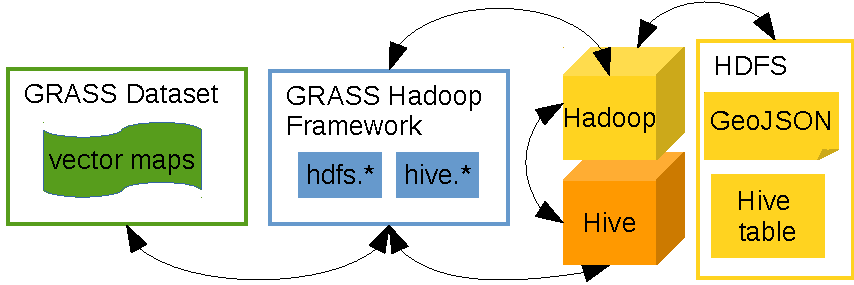
\includegraphics[width=1\textwidth]{./img/ghf_overview.pdf}
    \caption[Components interaction]{\centering Components interaction}
 \end{figure} 
\subsubsection{GRASS HDFS interface}
The modules start with \textit{hdfs.*}(exclude \textit{hdfs.db.connection}) provide tools for transferring data between GRASS maps or filsystem and Hadoop distributed file system. In addition the module \textit{hdfs.info} provide basic metadata of files stored in HDFS.

\paragraph{HDFS metadata} Module \textit{hdfs.info} currently support several basic operation for checking if path exist, recursive listing of directories and creating HDFS directory.

%TODO run cluster and show output

\paragraph{GRASS Map to HDFS} Vector maps in native GRASS format are not suitable for serialisation which is needed to exploiting the potential of spatial frameworks for Hadoop. The effective way, and in the most cases the only possible is to store spatial data in JSON, especially GeoJSON. This format is well suited for serialisation and function for reading it is in standard catalogue of Hive. 

Module \textit{hdfs.in.vector} supports transformation of GRASS map to HDFS in GeoJSON format. The behind the module are two main steps. Firstly, map is converted to GeoJSON using \textit{v.out.ogr} and edited to format which is suitable for parsing by widely known SerDe functions for Hive. After that, custom GeoJSON format is uploaded to the  destination on HDFS. By default, the HDFS path is set to \textit{hdfs://grass\_data\_hdfs/\textless LOCATION\_NAME \textgreater/\textless MAPSET \textgreater /vector}.

In addition, hdfs.* package also include module \textit{hdfs.in.fs} which allows to transfer external files to HDFS. Usage of this module came important for uploading CSV  or GeoJSON files. For uploading external GoeJSON files to HDFS is necessary to modify its standardised format. The serialiser\ref{serialiser}  for JSON has several format requirements. %TODO add ref

\begin{itemize}
\item Each vector feature must be on separated/new line.
\item brackets must be at the same line.
\begin{footnotesize}
\begin{lstlisting}[style=python]
// this will work
{ "key" : 10 }

// this will not work
{
  "key" : 10 
}
\end{lstlisting}
\end{footnotesize}

%{footnotesize}
\item header of GeoJSON must be erased. For GeoJSON exported by \textit{v.out.ogr} means to remove first 5 lines and last 3.
\begin{footnotesize}
\begin{lstlisting}[style=python]
//GeoJSON format. Not possible to serialise
{
"type": "FeatureCollection",
"crs": { "type": "name", "properties": { "name": "urn:ogc:def...
                                                                                
"features": [
{ "type": "Feature", "properties": { "cat": 546 }, "geometry":...
{ "type": "Feature", "properties": { "cat": 539 }, "geometry":...
]
}

// possible to serialise
{ "type": "Feature", "properties": { "cat": 546 }, "geometry":...
{ "type": "Feature", "properties": { "cat": 539 }, "geometry":...
\end{lstlisting}
\end{footnotesize}
\end{itemize}



\paragraph{HDFS GeoJSON to GRASS map}
To bring results back from HDFS is ensured by module \textit{hdfs.out.vector}. The module download deserialised GeoJSON file from HDFS and in second step modify file to standard GeoJSON format. The second step is important to make file consistent according to GeoJSON standard. In that time, format is readable by \textit{v.in.ogr} which is based on GDAL/OGR library and can be transformed to the native vector map format.

\subsubsection{GRASS Hive interface}
Two spatial frameworks, from ESRI and HadoopGIS use Hive as a top layer for usage map reduce based library in more expressive way. The GRASS Hadoop Framework consist several modules starts with prefix hive.* analogically to mentioned hdfs.* modules. Module for connection to Hive is covered by module \textit{hdfs.db.connect} which is an exception in naming nomenclature. The "hive" modules provide functions for creating tables and loading data into. Furthermore is available module for select queries and execute commands. Main two modules \textit{hive.csv.table} and \textit{hive.json.table} support user friendly creation of tables and loading data into. The process of creation table and loading data can be split. The hive.*.table modules support creation table without loading data. This step can be provided by module hive.table.load or simply by Hive command using hive.execute.


\paragraph{Creation of table} Spatial framework from Esri supports reading  from several file format.  The Framework allows to create geometric data type from  WKB, JSON and GeoJSON. Table can be crated from \textit{hiveserver2} command line or with using developed module  \textit{hive.json.table} within GHF.D Defining feature of table is provided using parameters and flags of module. It module to user make table with GeoJSON table without advanced knowledges of Hive syntax. In table \ref{hive.json} are described main features of each parameter. The examples of usage are shown in the next section\ref{sec:usage_spatial}. Second, slightly modified module supports creation of table suited for loading CSV data. In hive.* package is also module for loading data to table. This module is not necessary used, because is build-in for hdfs.*.table modules. 



\begin{table}[!htbp]
\begin{footnotesize}
\centering
\begin{tabular}{@{}|l|l||l|l|@{}}
\toprule
parameter  & description                                                                                                                & flag & description                  \\ \midrule  \midrule
driver     & \begin{tabular}[c]{@{}l@{}}Type of database driver\\ options:\\ hive\_cli,hiveserver2,\end{tabular}                        & -e   & create external table        \\ \midrule
table      & name of table                                                                                                              & -o   & overwrite data in table      \\ \midrule
attributes & \begin{tabular}[c]{@{}l@{}}python dictionary\\ \{attribute:datatype\}\end{tabular}                                         & -d   & Firstly drop table if exists \\ \midrule
struct     & structure of json                                                                                                          &      &                              \\ \midrule
stored     & output format                                                                                                              &      &                              \\ \midrule
serde      & \begin{tabular}[c]{@{}l@{}}java class for serialization of json\\ default: org.openx.data.jsonserde.JsonSerDe\end{tabular} &      &                              \\ \midrule
outformat  & java class for handling output format                                                                                      &      &                              \\ \midrule
jsonpath   & hdfs path specifying input data                                                                                            &      &                              \\ \bottomrule
\end{tabular}
\caption{Description of \textit{hive.json.table} parameters and flags}
\label{hive.json}
\end{footnotesize}
\end{table}

\paragraph{Select and execute} In package are two additional modules for advanced commands. The module \textit{hive.select} allows to build custom query and give the result to standard out or to the file. The second one, module for execution can be used for any command but working properly only with non-optimised query type, as creating table, loading data, dropping databases etc. Thus queries without complex output result.


\begin{figure}[!htbp]
   \centering
   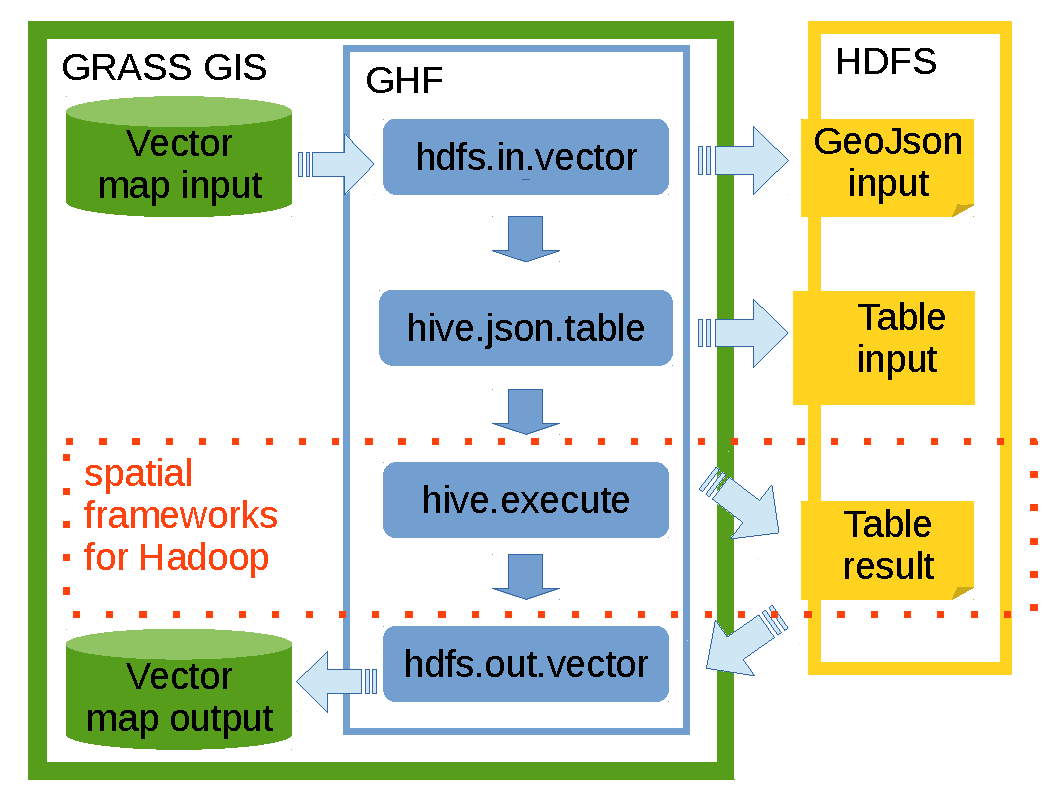
\includegraphics[width=0.8\textwidth]{./img/modules_schema.pdf}
   \caption[GHF workflow]{\centering Process workflow of GRASS Hadoop Framework  }
\end{figure} 
 
\subsection{Implementation}
Package GRASS Hadoop Framework has been developed in python language. The background of the choice of python language is fact, that GRASS GIS natively supports python and is fully covered by  API. As GRASS GIS modular design, the user interface of package GRASS Hadoop Framework is modular as well. The user interface is provided by command line modules. 
The design of framework is based on several layers. The core library, the middle interface and the top level interface. The core library of this project are wrappers for HDFS and Hive drivers and its management of connection. The middle interface are factories for the top level interface, thus modules  accessible from GRASS GIS user interface.

  \begin{figure}[!htbp]
   \centering
   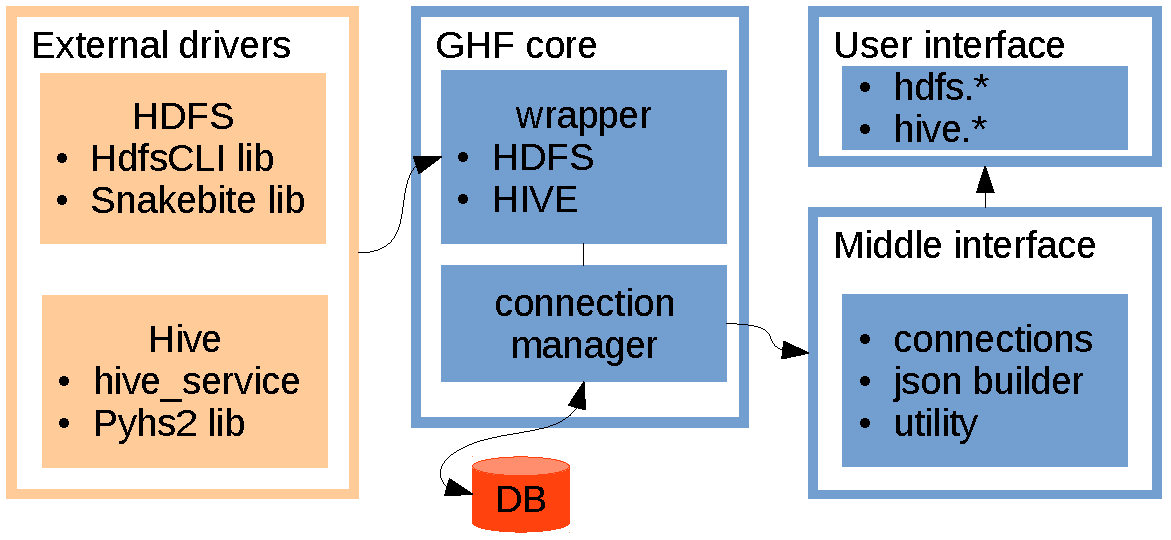
\includegraphics[width=1\textwidth]{./img/implementation.pdf}
   \caption[Architecture of GHF]{\centering Architecture of GRASS Hadoop Framework}
\end{figure} 
 
 
\subsection{External libraries(drivers)}
In this section are introduced the external libraries for interaction with HDFS and Hive which are used in GHF. 

\paragraph{HDFS libraries}
For communication with HDFS are used two libraries. First, wrapper of \textit{HdfsCLI} command line shell wchich is primary developed to makes interaction with HDFS more intuitive than standard \textit{hadoop fs} command line shell. It  has features as completion, command history and ANSI formatting. For this tools is implemented wrapper as a python library. The controlling of remote HDFS is based on WebHDFS REST API and HttpFS supporting both secure and insecure clusters.

Second library which has been developed for Spotify project, is called Snakebite. This library is as well as first shared under Apache licence, Version 2.0. The library is written as pure HDFS client to eliminate expensive calling \textit{hadoop} from python. The HDFS client instead of calling hadoop use Protocol Buffers, which  are a language-neutral, platform-neutral extensible mechanism for serializing structured data.\cite{protobuf}. Snakebite relay on protobuf messages and implements the Hadoop RPC protocol description for talking to the NameNode.\cite{snakebite}

\paragraph{Hive libraries}
As for HDFS for interaction with Hive has been used two libraries. The first, called \textit{pyhs2} for interaction with hiveserver2. It includes all the required packages such as SASL and Thrift wrappers. The second used library is \textit{hive-thrift-py}. From this Thrift based library has been used module for accessing meta-store of Hive.

\subsection{GHF core}
The core provide API for the middle interface. Consists functions for interaction with HDFS and Hive database. More specifically, allows to put/get data to/from HDFS and interact with HDFS using essential file system commands. The part focused on Hive interaction, allows to create specific table for loading CSV and JSON files, fetch metadata from meta store of Hive, and execute non-optimised queries or fetch result of select query. In the core library is used part of the code from \textit{Airflow} project, which is currently in incubator of Apache\footnote{\textit{airflow.diff} of code is in attachment}. The core library are mainly wrappers on the mentioned external libraries. The classes of core library can be parted to the  wrappers(hooks) and to the connection manager. 

\begin{figure}[!htbp]
   \centering
   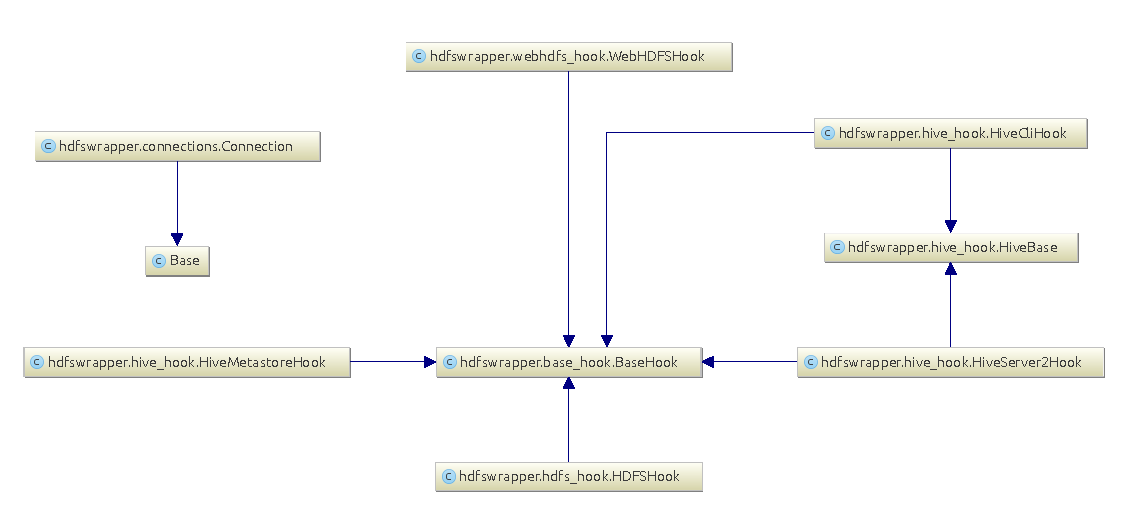
\includegraphics[width=1\textwidth]{./img/diag1_small.pdf}
   \caption[Core diagram]{\centering Diagram of core library classes}
\end{figure} 

\paragraph{Connection} management on the  lower level is handled by  class \textit{Connection}. The class is an place holder to store information about different database instances. The class inherits the  base class for declarative class definitions of SQLAlchemy library. 
It allows to use ORM SQL in expressive/programmatically way.  
\begin{footnotesize}
\begin{lstlisting}[style=python]
from sqlalchemy.ext.declarative import declarative_base
Base = declarative_base()

class Connection(Base):
    __tablename__ = "connection"
    id = Column(Integer(), primary_key=True)
    conn_id = Column(String(ID_LEN),unique=True)
    conn_type = Column(String(500))
\end{lstlisting}
\end{footnotesize}
The class ensure integrity of initialisation of \textit{connection} table in database and the main access point for getting hooks of each connection type, such a hdfs hook, hive hook etc. 
\begin{footnotesize}
\begin{lstlisting}[style=python]
def get_hook(self):
	"""End point for accessing hooks"""
    if self.conn_type == 'hiveserver2':
    		return hive_hook.HiveServer2Hook(HiveServer2Hook=self.conn_id)
    elif self.conn_type == 'webhdfs':
        return webhdfs_hook.WebHDFSHook(webhdfs_conn_id=self.conn_id)
\end{lstlisting}
\end{footnotesize}
After initialisation instance of the \textit{Connection} class the method \textit{get\_hook} return connection hook according class variable \textit{conn\_id}, which is an unique identifier for each group of connection type, such as \textit{hiveserver2}, \textit{webhdfs} etc.

\paragraph{Connection hooks}
Python modules called \textit{*\_hook.py} consist classes which inherits from the class \textit{BaseHook} stored in module \textit{base\_hook.py}.
\textit{BaseHook} is an abstract class for hooks and return object that can handle the connection and interaction to specific instances of these systems, and expose consistent methods to interact with them.

Modules \textit{*\_hook.py} and their hook classes provide wrappers on the external libraries. Module \textit{hdfs\_hook.py} and \textit{webhdfs\_hook.py} provide essential functions as put data to HDFS, get data from HDFS, make directory, check if path exists etc. 
The module \textit{ hive\_hook.py} consist three classes. The class \textit{HiveServer2Hook} allows to interact with \textit{hiveserver2} cli. The second class is a simple wrapper around the hive CLI. It allso support beeline Hive CLI, which is lighter due to independence on JDBC. Third class of this module -  \textit{HiveMetastoreHook} provide access to meta store of Hive. 


These hook are API for the middle interface which is introduced in the next section.


\section{Usage: Spatial data processing}\label{sec:usage_spatial}
	\subsection{Input data}

	
	Note that the 2.3.2 sandbox does not have a directory in HDFS for the root user and this can cause Hive queries to fail. To remedy this you need to issue the following commands as root:
su hdfs
hdfs dfs -mkdir /user/root
hdfs dfs -chown root:hdfs /user/root
exit
	



http://stackoverflow.com/questions/31802908/adding-hive-jars-permanently
In the hiveserver2 host, create a location something like /var/lib/hive and add all the necessary jars inside that folder. Edit the hive-site.xml and mention all these jars in the property hive.aux.jars.path

Eg: ADD JAR /home/amal/hive/amaludf.jar ADD JAR /home/amal/hive/amaludf2.jar

Instead of using the above commands in each session, you can define it for all sessions.

Create a location for storing these jars in the hiveserver host.

mkdir /var/lib/hive
Add all these jars to that directory

Set the property in hive-site.xml

<property>
  <name>hive.aux.jars.path</name>
  <value>/var/lib/hive</value>
</property>
Restart the hiveserver2 after doing this modification.

Instead of creating a directory and putting all the jars, you can specify paths of individual jars also. The only condition is that all these jars should be present in the hiveserver host.

Eg:

<property>
  <name>hive.aux.jars.path </name>
  <value>file:///home/amal/hive/udf1.jar,file:///usr/lib/hive/lib/hive-hbase-handler.jar</value>
</property>
	
		\subsubsection{CSV}
		
		https://community.hortonworks.com/articles/2834/when-to-use-and-when-not-to-use-hive-csvserde.html
		\subsubsection{GeoJSON}\label{json}	
			\paragraph{Standard GeoJSON}	
			\paragraph{ESRI GeoJSON}
				\begin{enumerate}
					\item[Enclosed]
					\item[Unenclosed]
				\end{enumerate}
	
	
	\subsection{Storing data}
	external table
	load from local


	\paragraph{HIVE}
	https://cwiki.apache.org/confluence/display/Hive/DeveloperGuide
	STORED AS TEXTFILE	
STORED AS INPUTFORMAT
  'org.apache.hadoop.mapred.TextInputFormat'
  OUTPUTFORMAT
  'org.apache.hadoop.hive.ql.io.IgnoreKeyTextOutputFormat'
	
	
	What is a SerDe?
SerDe is a short name for "Serializer and Deserializer."
Hive uses SerDe (and FileFormat) to read and write table rows.
HDFS files --> InputFileFormat --> <key, value> --> Deserializer --> Row object
Row object --> Serializer --> <key, value> --> OutputFileFormat --> HDFS files

	
	Metastore server describe
	
	
	
	\subsection{Query data}
	Hive vs Postges vs BigQuery
	
	

			
		
	
\section{}



\chapter*{}\stepcounter{chapter}\addcontentsline{toc}{chapter}{}

\pagenumbering{gobble}
\newpage
\necislovana{Acronyms}
\begin{acronym}
 \setlength{\parskip}{0ex}
 \setlength{\itemsep}{1ex}
  	\acro{API}{Application Programming Interface}
  	\acro{CSV}{Comma Separated Values}

  	\acro{EPSG}{Geodetic Parameter Set}	
  	
  	\acro{GIS}{Geographic Information System}
  	\acro{GNU GPL}{GNU General Public License } 
	\acro{GRASS}{Geographical Resources Analysis Support System}
	\acro{GUI}{Graphical User Interface}

\end{acronym}




\newpage
\renewcommand\baselinestretch{1.2}
\selectfont
\renewcommand{\refname}{References}
\phantomsection
\addcontentsline{toc}{section}{ \refname}

\begin{thebibliography}{99}
\label{References}



\bibitem{hadoop_definitive}
WHITE, Tom. \textit{Hadoop: the definitive guide. Fourth edition.} Beijing: O'Reilly, 2015. ISBN 14-919-0163-2.

\bibitem{kerberos}
NEUMAN, B.C. a T. TS'O. \textit{Kerberos. IEEE Communications Magazine}. 1994, 32(9). DOI: 10.1109/35.312841. ISSN 0163-6804.  URL: \textless\url{http://ieeexplore.ieee.org/lpdocs/epic03/wrapper.htm?arnumber=312841}


\bibitem{spatial_join}
JACOX, Edwin H. a Hanan SAMET. \textit{Spatial join techniques}. ACM Transactions on Database Systems. 2007, 32(1), 1-5. DOI: 10.1145/1206049.1206056. ISSN 03625915. URL: \textless\url{http://portal.acm.org/citation.cfm?doid=1206049.1206056}

\bibitem{partitioning}
Ablimit Aji, Vo Hoang, Fusheng Wang \textit{Effective Spatial Data Partitioning for Scalable Query Processing} 2015/9/3,
Journal: arXiv preprint arXiv:1509.00910 \textless\url{http://arxiv.org/pdf/1509.00910}

\bibitem{spatial_skew}
Ray, Suprio, et al. \textit{Skew-resistant parallel in-memory spatial join.} Proceedings of the 26th International Conference on Scientific and Statistical Database Management. ACM, 2014.

\bibitem{spatial_join2}
YOU, Simin, Jianting ZHANG a Le GRUENWALD. \textit{Large-scale spatial join query processing in Cloud.} 2015 31st IEEE International Conference on Data Engineering Workshops. IEEE, 2015, , 34-41. DOI: 10.1109/ICDEW.2015.7129541. ISBN 978-1-4799-8442-8. URL: \textless\url{http://ieeexplore.ieee.org/lpdocs/epic03/wrapper.htm?arnumber=7129541}

\bibitem{covex_hull}
GOMES, Abel J.P. A \textit{Total Order Heuristic-Based Convex Hull Algorithm for Points in the Plane. Computer-Aided Design.} 2016, 70, 153-160. DOI: 10.1016/j.cad.2015.07.013. ISSN 00104485.  URL: \textless\url{http://linkinghub.elsevier.com/retrieve/pii/S001044851500113X}

\bibitem{omp}
Wirz, Alexander, Björn Knafla, and Claudia Leopold. \textit{Comparison of Spatial Data Structures in OpenMP-Parallelized Steering.} HIGH PERFORMANCE COMPUTING  SIMULATION (HPCS 2008) (2008): 31.

\bibitem{multi_cpu}
ZHANG, Jianting, Simin YOU a Le GRUENWALD. \textit{Parallel online spatial and temporal aggregations on multi-core CPUs and many-core GPUs.} Information Systems. 2014, 44, 134-154. DOI: 10.1016/j.is.2014.01.005. ISSN 03064379.URL:  \textless\url{http://linkinghub.elsevier.com/retrieve/pii/S0306437914000234}


\bibitem{hadoopGIS}
AJI, Ablimit, Fusheng WANG, Hoang VO, Rubao LEE, Qiaoling LIU, Xiaodong ZHANG a Joel SALTZ. \textit{Hadoop GIS:A High Performance Spatial Data Warehousing System over MapReduce.} 2013, 6(11), 1009-1020. DOI: 10.14778/2536222.2536227. ISSN 21508097.  URL:  \textless\url{http://dl.acm.org/citation.cfm?doid=2536222.2536227}

\bibitem{spatialhadoop}
ELDAWY, Ahmed a Mohamed F. MOKBEL. \textit{SpatialHadoop: A MapReduce framework for spatial data.} DOI: 10.1109/ICDE.2015.7113382. ISBN 10.1109/ICDE.2015.7113382. URL:  \textless\url{http://ieeexplore.ieee.org/lpdocs/epic03/wrapper.htm?arnumber=7113382}

\bibitem{esri_indexing}
WHITMAN, Randall T., Michael B. PARK, Sarah M. AMBROSE a Erik G. HOEL. \textit{Spatial indexing and analytics on Hadoop.} Proceedings of the 22nd ACM SIGSPATIAL International Conference on Advances in Geographic Information Systems - SIGSPATIAL '14. New York, New York, USA: ACM Press, 2014, , 73-82. DOI: 10.1145/2666310.2666387. ISBN 9781450331319. URL:  \textless\url{http://dl.acm.org/citation.cfm?doid=2666310.2666387}

\bibitem{spatial_indexing}
FOX, Anthony, Chris EICHELBERGER, James HUGHES a Skylar LYON. \textit{Spatio-temporal indexing in non-relational distributed databases.} 2013 IEEE International Conference on Big Data. IEEE, 2013, , 291-299. DOI: 10.1109/BigData.2013.6691586. ISBN 978-1-4799-1293-3. URL:  \textless\url{http://ieeexplore.ieee.org/lpdocs/epic03/wrapper.htm?arnumber=6691586}

\bibitem{google_fs}
GHEMAWAT, Sanjay, Howard GOBIOFF a Shun-Tak LEUNG. \textit{The Google file system. ACM SIGOPS Operating Systems Review.} 2003, 37(5), 29-. DOI: 10.1145/1165389.945450. ISSN 01635980.  URL:  \textless\url{http://portal.acm.org/citation.cfm?doid=1165389.945450}

\bibitem{lisp}
DEAN, Jeffrey a Sanjay GHEMAWAT. \textit{MapReduce: Simplified Data Processing on Large Clusters}  2008, 51(1), 107-. DOI: 10.1145/1327452.1327492. ISSN 00010782. URL:  \textless\url{http://static.googleusercontent.com/media/research.google.com/en//archive/mapreduce-osdi04.pdf}



%%%%%%% online
\bibitem{permission}
HDFS Permissions Guide, Apache Hadoop  [online]. [2016-05-06]. URL:  \textless\url{https://hadoop.apache.org/docs/current/hadoop-project-dist/hadoop-hdfs/HdfsPermissionsGuide.html}

\bibitem{esri_framework}
GIS Tools for Hadoop. Esri GitHub [online]. [2016-03-18]. URL:  \textless\url{http://esri.github.io/gis-tools-for-hadoop/}

\bibitem{rest_api}
WebHDFS REST API, Apache Hadoop  [online]. [2016-05-06]. URL:  \textless\url{http://hadoop.apache.org/docs/current/hadoop-project-dist/hadoop-hdfs/WebHDFS.html#Append_to_a_File
}

\bibitem{amazon_emr}
Amazon EMR. Amazon [online]. [2016-03-18]. 
URL: \textless\url{https://aws.amazon.com/elasticmapreduce/}

\bibitem{hadoop_web}
Apache Hadoop main. Apache Hadoop [online]. [2016-03-18]. 
URL: \textless\url{http://hadoop.apache.org/}

\bibitem{nutch_web}
Apache Nutch. Apache Hadoop [online]. [2016-03-18]. 
URL: \textless\url{http://nutch.apache.org/#News
}

\bibitem{hadoop_news_web}
Apache Hadoop news. Apache Hadoop [online]. [2016-03-18]. 
URL: \textless\url{http://hadoop.apache.org/index.html#News}


\bibitem{hadoop_hdfs_web}
Apache Hadoop news. Apache Hadoop [online]. [2016-03-18]. 
URL: \textless\url{https://hadoop.apache.org/docs/r1.2.1/hdfs_design.html}


\bibitem{hadoop_rack_web}
Hadoop Rack Awareness. Apache Hadoop [online]. [2016-03-18]. 
URL: \textless\url{https://hadoop.apache.org/docs/r1.2.1/cluster_setup.html#Hadoop+Rack+Awareness}

\bibitem{gc_hadoop}
Google Cloud, Hadoop Configuration [online]. [2016-04-18]. 
URL: \textless\url{https://cloud.google.com/hadoop/setting-up-a-hadoop-cluster#setupscripts}

\bibitem{yarn}
Apache Hadoop docs. Apache Hadoop [online]. [2016-05-18]. 
URL: \textless\url{https://hadoop.apache.org/docs/r2.7.1/hadoop-yarn/hadoop-yarn-site/YARN.html}

\bibitem{hadoop}
Apache Hadoop setting up Single cluster node, Apache Hadoop [online]. [2016-05-18]. 
URL: \textless\url{https://hadoop.apache.org/docs/r2.7.1/hadoop-yarn/hadoop-yarn-site/YARN.html}


\bibitem{esri_gtfp}
Geoprocessing Tools for Hadoop, GitHub. [online]. [2016-05-18]. 
URL: \textless\url{https://github.com/Esri/geoprocessing-tools-for-hadoopl}

\bibitem{protobuf}
Protocol Buffers, Google Developers [online]. [2016-05-29]. 
URL: \textless\url{https://developers.google.com/protocol-buffers/}

\bibitem{snakebite}
Snakebite documentation, Snakebite readthedocs [online]. [2016-05-29]. 
URL: \textless\url{http://snakebite.readthedocs.io/en/latest/index.html
}

\end{thebibliography}




\setcounter{footnote}{1}
\newpage

\appendix
\chapter*{Attachment}
\renewcommand\thesection{\Alph{section}}

\section{Attachment:python script for SQL export}
\section{priloha 123}

\end{document}









